\documentclass[11pt,a4paper]{article}

\usepackage[margin=18.5mm,top=21mm,bottom=18mm]{geometry}
\usepackage{amsmath,amssymb,amsthm,mathtools}
\usepackage{booktabs,array}
\usepackage{enumitem}
\usepackage{xcolor}
\usepackage{fancyhdr}
\usepackage{graphicx}
\usepackage{tikz}
\usetikzlibrary{arrows.meta,calc,positioning,patterns,plotmarks}
\usepackage[hidelinks]{hyperref}

\graphicspath{{figures/}}
\newcommand{\pOneConvFirst}{(0.42114,2.79845) (2.00827,3.14326) (3.59540,3.47601) (5.18253,3.78234)}
\newcommand{\pOneConvTvd}{(0.42114,0.77470) (2.00827,1.26718) (3.59540,1.75007) (5.18253,2.22307)}
\newcommand{\pOneConvEnoTwo}{(0.42114,1.57790) (2.00827,2.01740) (3.59540,2.44488) (5.18253,2.85681)}
\newcommand{\pOneConvEnoThree}{(0.42114,1.01844) (2.00827,1.50313) (3.59540,1.97308) (5.18253,2.43237)}
\newcommand{\pOneConvWenoThree}{(0.42114,1.07950) (2.00827,1.60266) (3.59540,2.10492) (5.18253,2.57939)}
\newcommand{\pOneConvWenoFive}{(0.42114,0.30254) (2.00827,0.86591) (3.59540,1.41998) (5.18253,1.95646)}
\newcommand{\pOneSlopeHalf}{(0.42114,2.64716) (5.18253,3.73687)}
\newcommand{\pOneSlopeTwoThirds}{(0.42114,1.10683) (5.18253,2.55977)}
\newcommand{\pOneSlopeFiveSixths}{(0.42114,0.19109) (5.18253,2.00727)}
\newcommand{\pTwoConvFirst}{(0.48139,3.71123) (1.97674,3.82230) (3.47209,3.90401) (4.96744,3.95679)}
\newcommand{\pTwoConvTvd}{(0.48139,2.59423) (1.97674,3.00232) (3.47209,3.36100) (4.96744,3.69513)}
\newcommand{\pTwoConvEnoTwo}{(0.48139,2.93759) (1.97674,3.33398) (3.47209,3.65042) (4.96744,3.82890)}
\newcommand{\pTwoConvEnoThree}{(0.48139,2.02065) (1.97674,2.60447) (3.47209,3.20809) (4.96744,3.65519)}
\newcommand{\pTwoConvWenoThree}{(0.48139,2.27571) (1.97674,2.92777) (3.47209,3.46633) (4.96744,3.76669)}
\newcommand{\pTwoConvWenoFive}{(0.48139,0.18240) (1.97674,1.55153) (3.47209,2.57149) (4.96744,3.35096)}
\newcommand{\pTwoSlopeTwo}{(0.48139,2.49389) (4.96744,3.89197)}
\newcommand{\pTwoSlopeThree}{(0.48139,1.95285) (4.96744,4.04997)}
\newcommand{\pTwoSlopeFive}{(0.48139,0.17172) (3.47209,2.50186)}
\newcommand{\pTwoWorkFirst}{(0.24920,3.95679) (1.17278,3.90401) (2.21151,3.82230) (3.58057,3.71123)}
\newcommand{\pTwoWorkTvd}{(0.80655,3.69513) (1.73689,3.36100) (2.80339,3.00232) (4.05247,2.59423)}
\newcommand{\pTwoWorkEnoTwo}{(0.79482,3.82890) (1.70557,3.65042) (2.72611,3.33398) (3.96672,2.93759)}
\newcommand{\pTwoWorkEnoThree}{(1.14723,3.65519) (2.14328,3.20809) (3.26152,2.60447) (4.57234,2.02065)}
\newcommand{\pTwoWorkWenoThree}{(1.44080,3.76669) (2.34107,3.46633) (3.39603,2.92777) (4.62769,2.27571)}
\newcommand{\pTwoWorkWenoFive}{(1.56211,3.35096) (2.63239,2.57149) (3.84244,1.55153) (5.17063,0.18240)}
\newcommand{\pThreeConvFirst}{(0.49190,1.02524) (2.01987,2.15569) (3.54784,2.96615) (5.07581,3.65701)}
\newcommand{\pThreeConvTvd}{(0.49190,0.52047) (2.01987,0.36590) (3.54784,1.53901) (5.07581,2.43470)}
\newcommand{\pThreeConvEnoTwo}{(0.49190,0.52061) (2.01987,0.36630) (3.54784,1.53891) (5.07581,2.43471)}
\newcommand{\pThreeConvEnoThree}{(0.49190,1.27637) (2.01987,1.31961) (3.54784,1.98639) (5.07581,2.67512)}
\newcommand{\pThreeConvWenoThree}{(0.49190,1.32349) (2.01987,1.37414) (3.54784,2.15074) (5.07581,2.76253)}
\newcommand{\pThreeConvWenoFive}{(0.49190,2.28766) (2.01987,2.32675) (3.54784,2.57369) (5.07581,2.94786)}
\newcommand{\pThreeSlopeOne}{(0.49190,0.87752) (5.07581,3.31959)}

\newcommand{\pOneSliceExact}{(-0.36000,0.00000) (-0.14142,0.00000) (-0.14142,1.00000) (0.14142,1.00000) (0.14142,0.00000) (0.36000,0.00000)}
\newcommand{\pOneSliceFirst}{(-0.35576,0.00000) (-0.32925,0.00000) (-0.30273,0.00000) (-0.27621,0.00006) (-0.24970,0.00107) (-0.23644,0.00354) (-0.22760,0.00731) (-0.22318,0.01028) (-0.21876,0.01425) (-0.21434,0.01948) (-0.20992,0.02624) (-0.20550,0.03485) (-0.20108,0.04566) (-0.19666,0.05900) (-0.19224,0.07522) (-0.18783,0.09462) (-0.18341,0.11748) (-0.17899,0.14399) (-0.17457,0.17426) (-0.17015,0.20828) (-0.16573,0.24592) (-0.16131,0.28693) (-0.15689,0.33092) (-0.15247,0.37737) (-0.14805,0.42566) (-0.14363,0.47509) (-0.13921,0.52491) (-0.13479,0.57434) (-0.13037,0.62263) (-0.12595,0.66908) (-0.12153,0.71307) (-0.11711,0.75408) (-0.11270,0.79172) (-0.10828,0.82574) (-0.10386,0.85601) (-0.09944,0.88252) (-0.09502,0.90538) (-0.09060,0.92478) (-0.08618,0.94100) (-0.08176,0.95434) (-0.07734,0.96515) (-0.07292,0.97376) (-0.06850,0.98052) (-0.06408,0.98575) (-0.05966,0.98972) (-0.05524,0.99269) (-0.05082,0.99487) (-0.04198,0.99759) (-0.01989,0.99972) (0.00663,0.99992) (0.03315,0.99893) (0.04640,0.99646) (0.05524,0.99269) (0.05966,0.98972) (0.06408,0.98575) (0.06850,0.98052) (0.07292,0.97376) (0.07734,0.96515) (0.08176,0.95434) (0.08618,0.94100) (0.09060,0.92478) (0.09502,0.90538) (0.09944,0.88252) (0.10386,0.85601) (0.10828,0.82574) (0.11270,0.79172) (0.11711,0.75408) (0.12153,0.71307) (0.12595,0.66908) (0.13037,0.62263) (0.13479,0.57434) (0.13921,0.52491) (0.14363,0.47509) (0.14805,0.42566) (0.15247,0.37737) (0.15689,0.33092) (0.16131,0.28693) (0.16573,0.24592) (0.17015,0.20828) (0.17457,0.17426) (0.17899,0.14399) (0.18341,0.11748) (0.18783,0.09462) (0.19224,0.07522) (0.19666,0.05900) (0.20108,0.04566) (0.20550,0.03485) (0.20992,0.02624) (0.21434,0.01948) (0.21876,0.01425) (0.22318,0.01028) (0.22760,0.00731) (0.23202,0.00513) (0.24086,0.00241) (0.26296,0.00028) (0.28947,0.00001) (0.31599,0.00000) (0.34250,0.00000) (0.35576,0.00000)}
\newcommand{\pOneSliceTvd}{(-0.35576,0.00000) (-0.32925,0.00000) (-0.30273,0.00000) (-0.27621,0.00000) (-0.24970,0.00000) (-0.22318,0.00000) (-0.19666,0.00000) (-0.17015,0.00000) (-0.15247,0.02567) (-0.14805,0.15478) (-0.14363,0.37348) (-0.13921,0.62652) (-0.13479,0.84522) (-0.13037,0.97433) (-0.12595,1.00000) (-0.09944,1.00000) (-0.07292,1.00000) (-0.04640,1.00000) (-0.01989,1.00000) (0.00663,1.00000) (0.03315,1.00000) (0.05966,1.00000) (0.08618,1.00000) (0.11270,1.00000) (0.13037,0.97433) (0.13479,0.84522) (0.13921,0.62652) (0.14363,0.37348) (0.14805,0.15478) (0.15247,0.02567) (0.15689,0.00000) (0.18341,0.00000) (0.20992,0.00000) (0.23644,0.00000) (0.26296,0.00000) (0.28947,0.00000) (0.31599,0.00000) (0.34250,0.00000) (0.35576,0.00000)}
\newcommand{\pOneSliceEnoTwo}{(-0.35576,0.00000) (-0.32925,0.00000) (-0.30273,0.00000) (-0.27621,0.00000) (-0.24970,0.00000) (-0.22318,0.00000) (-0.19666,0.00018) (-0.17899,0.00432) (-0.17457,0.00874) (-0.17015,0.01706) (-0.16573,0.03209) (-0.16131,0.05809) (-0.15689,0.10102) (-0.15247,0.16857) (-0.14805,0.26942) (-0.14363,0.41166) (-0.13921,0.58834) (-0.13479,0.73058) (-0.13037,0.83143) (-0.12595,0.89898) (-0.12153,0.94191) (-0.11711,0.96791) (-0.11270,0.98294) (-0.10828,0.99126) (-0.10386,0.99568) (-0.09944,0.99794) (-0.07734,0.99997) (-0.05082,1.00000) (-0.02431,1.00000) (0.00221,1.00000) (0.02873,1.00000) (0.05524,1.00000) (0.08176,0.99992) (0.10386,0.99568) (0.10828,0.99126) (0.11270,0.98294) (0.11711,0.96791) (0.12153,0.94191) (0.12595,0.89898) (0.13037,0.83143) (0.13479,0.73058) (0.13921,0.58834) (0.14363,0.41166) (0.14805,0.26942) (0.15247,0.16857) (0.15689,0.10102) (0.16131,0.05809) (0.16573,0.03209) (0.17015,0.01706) (0.17457,0.00874) (0.17899,0.00432) (0.18341,0.00206) (0.20550,0.00003) (0.23202,0.00000) (0.25854,0.00000) (0.28505,0.00000) (0.31157,0.00000) (0.33809,0.00000) (0.35576,0.00000)}
\newcommand{\pOneSliceEnoThree}{(-0.35576,0.00000) (-0.32925,0.00000) (-0.30273,0.00000) (-0.27621,0.00000) (-0.24970,0.00000) (-0.22318,0.00000) (-0.19666,0.00000) (-0.17015,0.00142) (-0.16573,0.00417) (-0.16131,0.01166) (-0.15689,0.03072) (-0.15247,0.07600) (-0.14805,0.17567) (-0.14363,0.37149) (-0.13921,0.62851) (-0.13479,0.82434) (-0.13037,0.92400) (-0.12595,0.96929) (-0.12153,0.98834) (-0.11711,0.99583) (-0.11270,0.99858) (-0.08618,1.00000) (-0.05966,1.00000) (-0.03315,1.00000) (-0.00663,1.00000) (0.01989,1.00000) (0.04640,1.00000) (0.07292,1.00000) (0.09944,0.99996) (0.11711,0.99583) (0.12153,0.98834) (0.12595,0.96928) (0.13037,0.92400) (0.13479,0.82432) (0.13921,0.62853) (0.14363,0.37148) (0.14805,0.17567) (0.15247,0.07600) (0.15689,0.03072) (0.16131,0.01166) (0.16573,0.00417) (0.17015,0.00142) (0.19666,0.00000) (0.22318,0.00000) (0.24970,0.00000) (0.27621,0.00000) (0.30273,0.00000) (0.32925,0.00000) (0.35576,0.00000)}
\newcommand{\pOneSliceWenoThree}{(-0.35576,-0.00000) (-0.32925,-0.00000) (-0.30273,0.00000) (-0.27621,-0.00000) (-0.24970,0.00000) (-0.22318,-0.00000) (-0.19666,-0.00001) (-0.17015,-0.00137) (-0.16573,0.00220) (-0.16131,0.01224) (-0.15689,0.03493) (-0.15247,0.08415) (-0.14805,0.18791) (-0.14363,0.37972) (-0.13921,0.62058) (-0.13479,0.81228) (-0.13037,0.91594) (-0.12595,0.96511) (-0.12153,0.98778) (-0.11711,0.99780) (-0.11270,1.00137) (-0.08618,1.00001) (-0.05966,1.00000) (-0.03315,1.00000) (-0.00663,1.00000) (0.01989,1.00000) (0.04640,1.00000) (0.07292,1.00000) (0.09944,0.99995) (0.11711,0.99780) (0.12153,0.98778) (0.12595,0.96511) (0.13037,0.91594) (0.13479,0.81228) (0.13921,0.62058) (0.14363,0.37972) (0.14805,0.18791) (0.15247,0.08415) (0.15689,0.03493) (0.16131,0.01224) (0.16573,0.00220) (0.17015,-0.00137) (0.19666,-0.00001) (0.22318,-0.00000) (0.24970,0.00000) (0.27621,-0.00000) (0.30273,0.00000) (0.32925,-0.00000) (0.35576,-0.00000)}
\newcommand{\pOneSliceWenoFive}{(-0.35576,0.00000) (-0.32925,0.00000) (-0.30273,-0.00000) (-0.27621,-0.00000) (-0.24970,0.00000) (-0.22318,0.00000) (-0.19666,0.00000) (-0.17015,0.00002) (-0.15689,0.00344) (-0.15247,0.01493) (-0.14805,0.06325) (-0.14363,0.29654) (-0.13921,0.70346) (-0.13479,0.93675) (-0.13037,0.98507) (-0.12595,0.99656) (-0.12153,0.99927) (-0.09502,1.00000) (-0.06850,1.00000) (-0.04198,1.00000) (-0.01547,1.00000) (0.01105,1.00000) (0.03757,1.00000) (0.06408,1.00000) (0.09060,1.00000) (0.11711,0.99985) (0.12595,0.99656) (0.13037,0.98507) (0.13479,0.93675) (0.13921,0.70346) (0.14363,0.29654) (0.14805,0.06325) (0.15247,0.01493) (0.15689,0.00344) (0.16131,0.00073) (0.18783,-0.00000) (0.21434,0.00000) (0.24086,-0.00000) (0.26737,-0.00000) (0.29389,0.00000) (0.32041,-0.00000) (0.34692,0.00000) (0.35576,0.00000)}

\newcommand{\pTwoSliceExact}{(0.25156,-0.00001) (0.26719,-0.00017) (0.28281,-0.00083) (0.29844,-0.00281) (0.31094,-0.00637) (0.32031,-0.01095) (0.32656,-0.01521) (0.33281,-0.02061) (0.33594,-0.02377) (0.33906,-0.02724) (0.34219,-0.03102) (0.34531,-0.03511) (0.34844,-0.03949) (0.35156,-0.04413) (0.35469,-0.04898) (0.35781,-0.05400) (0.36094,-0.05911) (0.36406,-0.06424) (0.36719,-0.06928) (0.37031,-0.07411) (0.37344,-0.07860) (0.37656,-0.08259) (0.37969,-0.08590) (0.38594,-0.08976) (0.39531,-0.08537) (0.39844,-0.08028) (0.40156,-0.07298) (0.40469,-0.06326) (0.40781,-0.05089) (0.41094,-0.03568) (0.41406,-0.01745) (0.41719,0.00392) (0.42031,0.02855) (0.42344,0.05650) (0.42656,0.08778) (0.42969,0.12236) (0.43281,0.16014) (0.43594,0.20096) (0.43906,0.24462) (0.44219,0.29084) (0.44531,0.33928) (0.44844,0.38954) (0.45156,0.44118) (0.45469,0.49369) (0.45781,0.54654) (0.46094,0.59914) (0.46406,0.65089) (0.46719,0.70118) (0.47031,0.74938) (0.47344,0.79486) (0.47656,0.83705) (0.47969,0.87535) (0.48281,0.90925) (0.48594,0.93828) (0.48906,0.96202) (0.49219,0.98014) (0.49531,0.99236) (0.49844,0.99852) (0.50469,0.99236) (0.50781,0.98014) (0.51094,0.96202) (0.51406,0.93828) (0.51719,0.90925) (0.52031,0.87535) (0.52344,0.83705) (0.52656,0.79486) (0.52969,0.74938) (0.53281,0.70118) (0.53594,0.65089) (0.53906,0.59914) (0.54219,0.54654) (0.54531,0.49369) (0.54844,0.44118) (0.55156,0.38954) (0.55469,0.33928) (0.55781,0.29084) (0.56094,0.24462) (0.56406,0.20096) (0.56719,0.16014) (0.57031,0.12236) (0.57344,0.08778) (0.57656,0.05650) (0.57969,0.02855) (0.58281,0.00392) (0.58594,-0.01745) (0.58906,-0.03568) (0.59219,-0.05089) (0.59531,-0.06326) (0.59844,-0.07298) (0.60156,-0.08028) (0.60469,-0.08537) (0.60781,-0.08849) (0.62344,-0.08259) (0.62656,-0.07860) (0.62969,-0.07411) (0.63281,-0.06928) (0.63594,-0.06424) (0.63906,-0.05911) (0.64219,-0.05400) (0.64531,-0.04898) (0.64844,-0.04413) (0.65156,-0.03949) (0.65469,-0.03511) (0.65781,-0.03102) (0.66094,-0.02724) (0.66406,-0.02377) (0.66719,-0.02061) (0.67344,-0.01521) (0.67969,-0.01095) (0.68594,-0.00768) (0.69531,-0.00429) (0.71094,-0.00139) (0.72656,-0.00034) (0.74219,-0.00004) (0.74844,-0.00001)}
\newcommand{\pTwoSliceEightyFirst}{(0.25625,0.01205) (0.26875,0.01539) (0.28125,0.01945) (0.29375,0.02432) (0.30625,0.03009) (0.31875,0.03682) (0.33125,0.04457) (0.34375,0.05336) (0.35625,0.06315) (0.36875,0.07389) (0.38125,0.08541) (0.39375,0.09754) (0.40625,0.11000) (0.41875,0.12245) (0.43125,0.13450) (0.44375,0.14573) (0.45625,0.15568) (0.46875,0.16393) (0.48125,0.17008) (0.49375,0.17381) (0.50625,0.17489) (0.51875,0.17331) (0.53125,0.16916) (0.54375,0.16260) (0.55625,0.15391) (0.56875,0.14342) (0.58125,0.13156) (0.59375,0.11880) (0.60625,0.10560) (0.61875,0.09239) (0.63125,0.07958) (0.64375,0.06747) (0.65625,0.05631) (0.66875,0.04627) (0.68125,0.03742) (0.69375,0.02979) (0.70625,0.02334) (0.71875,0.01799) (0.73125,0.01363) (0.74375,0.01014)}
\newcommand{\pTwoSliceEightyTvd}{(0.25625,0.00001) (0.26875,0.00001) (0.28125,0.00001) (0.29375,-0.00108) (0.30625,-0.00898) (0.31875,-0.02099) (0.33125,-0.03378) (0.34375,-0.04520) (0.35625,-0.05361) (0.36875,-0.05800) (0.38125,-0.05914) (0.39375,-0.05907) (0.40625,-0.00711) (0.41875,0.12863) (0.43125,0.29193) (0.44375,0.44846) (0.45625,0.57647) (0.46875,0.66629) (0.48125,0.71793) (0.49375,0.73712) (0.50625,0.74082) (0.51875,0.73333) (0.53125,0.63514) (0.54375,0.47451) (0.55625,0.31138) (0.56875,0.17564) (0.58125,0.07811) (0.59375,0.01568) (0.60625,-0.01914) (0.61875,-0.03283) (0.63125,-0.03621) (0.64375,-0.03675) (0.65625,-0.03496) (0.66875,-0.02704) (0.68125,-0.01818) (0.69375,-0.01087) (0.70625,-0.00582) (0.71875,-0.00281) (0.73125,-0.00121) (0.74375,-0.00045)}
\newcommand{\pTwoSliceEightyEnoTwo}{(0.25625,-0.00356) (0.26875,-0.00591) (0.28125,-0.00827) (0.29375,-0.00990) (0.30625,-0.01078) (0.31875,-0.01103) (0.33125,-0.01087) (0.34375,-0.00932) (0.35625,-0.00470) (0.36875,0.00547) (0.38125,0.02501) (0.39375,0.05941) (0.40625,0.11595) (0.41875,0.20134) (0.43125,0.29085) (0.44375,0.36210) (0.45625,0.41322) (0.46875,0.44668) (0.48125,0.46552) (0.49375,0.47357) (0.50625,0.47544) (0.51875,0.47252) (0.53125,0.45616) (0.54375,0.41688) (0.55625,0.34655) (0.56875,0.25210) (0.58125,0.17113) (0.59375,0.10815) (0.60625,0.06296) (0.61875,0.03276) (0.63125,0.01362) (0.64375,0.00205) (0.65625,-0.00440) (0.66875,-0.00754) (0.68125,-0.00879) (0.69375,-0.00906) (0.70625,-0.00892) (0.71875,-0.00769) (0.73125,-0.00556) (0.74375,-0.00382)}
\newcommand{\pTwoSliceEightyEnoThree}{(0.25625,-0.00050) (0.26875,-0.00104) (0.28125,-0.00212) (0.29375,-0.00418) (0.30625,-0.00803) (0.31875,-0.01489) (0.33125,-0.02478) (0.34375,-0.03572) (0.35625,-0.04510) (0.36875,-0.05024) (0.38125,-0.04935) (0.39375,-0.03884) (0.40625,-0.01030) (0.41875,0.05094) (0.43125,0.16399) (0.44375,0.32185) (0.45625,0.49718) (0.46875,0.66171) (0.48125,0.78972) (0.49375,0.86132) (0.50625,0.86615) (0.51875,0.79844) (0.53125,0.66638) (0.54375,0.49315) (0.55625,0.31275) (0.56875,0.16552) (0.58125,0.06851) (0.59375,0.00942) (0.60625,-0.02389) (0.61875,-0.04058) (0.63125,-0.04658) (0.64375,-0.04504) (0.65625,-0.03734) (0.66875,-0.02638) (0.68125,-0.01627) (0.69375,-0.00957) (0.70625,-0.00548) (0.71875,-0.00306) (0.73125,-0.00167) (0.74375,-0.00089)}
\newcommand{\pTwoSliceEightyWenoThree}{(0.25625,0.00112) (0.26875,0.00063) (0.28125,-0.00113) (0.29375,-0.00482) (0.30625,-0.01085) (0.31875,-0.01904) (0.33125,-0.02817) (0.34375,-0.03590) (0.35625,-0.03922) (0.36875,-0.03563) (0.38125,-0.02336) (0.39375,0.00184) (0.40625,0.04838) (0.41875,0.13027) (0.43125,0.25727) (0.44375,0.39584) (0.45625,0.49922) (0.46875,0.56169) (0.48125,0.59647) (0.49375,0.61345) (0.50625,0.61793) (0.51875,0.61008) (0.53125,0.58545) (0.54375,0.53239) (0.55625,0.43292) (0.56875,0.28671) (0.58125,0.14658) (0.59375,0.05441) (0.60625,0.00156) (0.61875,-0.02760) (0.63125,-0.04241) (0.64375,-0.04727) (0.65625,-0.04339) (0.66875,-0.03331) (0.68125,-0.02110) (0.69375,-0.01037) (0.70625,-0.00294) (0.71875,0.00093) (0.73125,0.00202) (0.74375,0.00163)}
\newcommand{\pTwoSliceEightyWenoFive}{(0.25625,-0.00011) (0.26875,-0.00034) (0.28125,-0.00083) (0.29375,-0.00185) (0.30625,-0.00417) (0.31875,-0.00987) (0.33125,-0.02033) (0.34375,-0.03486) (0.35625,-0.05117) (0.36875,-0.06577) (0.38125,-0.07482) (0.39375,-0.07469) (0.40625,-0.05867) (0.41875,0.00061) (0.43125,0.13085) (0.44375,0.31626) (0.45625,0.52348) (0.46875,0.72007) (0.48125,0.87628) (0.49375,0.96498) (0.50625,0.96767) (0.51875,0.88179) (0.53125,0.72280) (0.54375,0.52052) (0.55625,0.31155) (0.56875,0.13106) (0.58125,0.00636) (0.59375,-0.05360) (0.60625,-0.07352) (0.61875,-0.07603) (0.63125,-0.06807) (0.64375,-0.05313) (0.65625,-0.03540) (0.66875,-0.01963) (0.68125,-0.00917) (0.69375,-0.00422) (0.70625,-0.00208) (0.71875,-0.00099) (0.73125,-0.00039) (0.74375,-0.00009)}

\newcommand{\pThreeCutFirst}{(-1.49687,0.78540) (-1.44687,0.78540) (-1.39687,0.78540) (-1.34688,0.78540) (-1.29688,0.78540) (-1.24687,0.78540) (-1.19687,0.78540) (-1.14687,0.78540) (-1.09687,0.82616) (-1.08437,2.24934) (-1.07187,4.40016) (-1.05937,4.64240) (-1.04688,4.69503) (-1.02187,4.74186) (-0.99687,4.78322) (-0.97187,4.82658) (-0.94687,4.87264) (-0.92188,4.92185) (-0.89687,4.97474) (-0.87187,5.03199) (-0.84687,5.09447) (-0.82187,5.16338) (-0.79688,5.24043) (-0.78437,5.28278) (-0.77187,5.32830) (-0.75937,5.37764) (-0.74687,5.43173) (-0.73438,5.49196) (-0.72187,5.56055) (-0.70937,5.64128) (-0.69687,5.74167) (-0.68437,5.87808) (-0.67188,6.09914) (-0.65937,6.80858) (-0.64687,9.71878) (-0.63437,10.89958) (-0.62187,10.98984) (-0.57187,10.99557) (-0.52187,10.99557) (-0.47187,10.99557) (-0.42188,10.99557) (-0.37187,10.99557) (-0.32187,10.99557) (-0.27188,10.99557) (-0.22187,10.99557) (-0.17188,10.99557) (-0.12187,10.99557) (-0.07187,10.99557) (-0.02187,10.99557) (0.02813,10.99545) (0.05313,10.73958) (0.06563,9.10413) (0.07812,7.93130) (0.09063,7.60172) (0.10313,7.44789) (0.11563,7.35124) (0.12813,7.28175) (0.14062,7.22790) (0.15313,7.18417) (0.17813,7.11604) (0.20312,7.06424) (0.22813,7.02283) (0.26562,6.97351) (0.31563,6.92326) (0.36563,6.88441) (0.41563,6.85316) (0.46563,6.82728) (0.51562,6.80535) (0.56563,6.78639) (0.61563,6.76965) (0.66563,6.75446) (0.71563,6.73541) (0.74063,6.66231) (0.75313,6.28433) (0.76562,2.72502) (0.77813,1.30235) (0.79063,1.09541) (0.80313,0.99770) (0.81563,0.93847) (0.82812,0.89832) (0.85313,0.84813) (0.90313,0.80382) (0.95312,0.79004) (1.00313,0.78639) (1.05313,0.78558) (1.10313,0.78543) (1.15313,0.78540) (1.20312,0.78540) (1.25313,0.78540) (1.30313,0.78540) (1.35313,0.78540) (1.40313,0.78540) (1.45312,0.78540) (1.49063,0.78540)}
\newcommand{\pThreeCutTvd}{(-1.49687,0.78540) (-1.44687,0.78540) (-1.39687,0.78540) (-1.34688,0.78540) (-1.29688,0.78540) (-1.24687,0.78540) (-1.19687,0.78540) (-1.14687,0.78540) (-1.09687,0.78540) (-1.07187,0.89722) (-1.05937,4.36980) (-1.04688,4.66757) (-1.02187,4.71399) (-0.98438,4.77493) (-0.95937,4.81888) (-0.93437,4.86582) (-0.90937,4.91615) (-0.88437,4.97039) (-0.85938,5.02918) (-0.83437,5.09346) (-0.80937,5.16474) (-0.78437,5.24551) (-0.77187,5.29079) (-0.75937,5.34062) (-0.74687,5.39673) (-0.73438,5.46237) (-0.72187,5.54437) (-0.70937,5.66130) (-0.69687,5.88283) (-0.68437,7.18597) (-0.67188,10.88216) (-0.65937,10.99426) (-0.60938,10.99557) (-0.55937,10.99557) (-0.50937,10.99557) (-0.45938,10.99557) (-0.40937,10.99557) (-0.35938,10.99557) (-0.30937,10.99557) (-0.25937,10.99557) (-0.20938,10.99557) (-0.15937,10.99557) (-0.10938,10.99557) (-0.05937,10.99557) (-0.00937,10.99557) (0.04063,10.99557) (0.09063,10.96831) (0.10313,8.99419) (0.11563,7.64751) (0.12813,7.41657) (0.14062,7.30807) (0.15313,7.23779) (0.16563,7.18569) (0.17813,7.14422) (0.20312,7.08033) (0.22813,7.03193) (0.26562,6.97639) (0.30313,6.93367) (0.35313,6.88928) (0.40313,6.85439) (0.45312,6.82602) (0.50313,6.80236) (0.55313,6.78227) (0.60313,6.76495) (0.65313,6.74989) (0.70312,6.73661) (0.75313,6.48327) (0.76562,1.52068) (0.77813,1.00187) (0.79063,0.88253) (0.80313,0.83248) (0.84063,0.78984) (0.89062,0.78550) (0.94063,0.78540) (0.99063,0.78540) (1.04063,0.78540) (1.09063,0.78540) (1.14062,0.78540) (1.19063,0.78540) (1.24063,0.78540) (1.29063,0.78540) (1.34063,0.78540) (1.39062,0.78540) (1.44063,0.78540) (1.49063,0.78540)}
\newcommand{\pThreeCutEnoTwo}{(-1.49687,0.78540) (-1.44687,0.78540) (-1.39687,0.78540) (-1.34688,0.78540) (-1.29688,0.78540) (-1.24687,0.78540) (-1.19687,0.78540) (-1.14687,0.78540) (-1.09687,0.78540) (-1.07187,0.89722) (-1.05937,4.36978) (-1.04688,4.66755) (-1.02187,4.71399) (-0.98438,4.77493) (-0.95937,4.81888) (-0.93437,4.86582) (-0.90937,4.91615) (-0.88437,4.97039) (-0.85938,5.02918) (-0.83437,5.09346) (-0.80937,5.16474) (-0.78437,5.24551) (-0.77187,5.29079) (-0.75937,5.34062) (-0.74687,5.39673) (-0.73438,5.46237) (-0.72187,5.54437) (-0.70937,5.66130) (-0.69687,5.88283) (-0.68437,7.18597) (-0.67188,10.88216) (-0.65937,10.99426) (-0.60938,10.99557) (-0.55937,10.99557) (-0.50937,10.99557) (-0.45938,10.99557) (-0.40937,10.99557) (-0.35938,10.99557) (-0.30937,10.99557) (-0.25937,10.99557) (-0.20938,10.99557) (-0.15937,10.99557) (-0.10938,10.99557) (-0.05937,10.99557) (-0.00937,10.99557) (0.04063,10.99557) (0.09063,10.96831) (0.10313,8.99422) (0.11563,7.64752) (0.12813,7.41658) (0.14062,7.30808) (0.15313,7.23781) (0.16563,7.18570) (0.17813,7.14423) (0.20312,7.08035) (0.22813,7.03195) (0.26562,6.97641) (0.30313,6.93370) (0.35313,6.88931) (0.40313,6.85442) (0.45312,6.82605) (0.50313,6.80240) (0.55313,6.78231) (0.60313,6.76498) (0.65313,6.74992) (0.70312,6.73664) (0.75313,6.48331) (0.76562,1.52082) (0.77813,1.00188) (0.79063,0.88253) (0.80313,0.83248) (0.84063,0.78984) (0.89062,0.78550) (0.94063,0.78540) (0.99063,0.78540) (1.04063,0.78540) (1.09063,0.78540) (1.14062,0.78540) (1.19063,0.78540) (1.24063,0.78540) (1.29063,0.78540) (1.34063,0.78540) (1.39062,0.78540) (1.44063,0.78540) (1.49063,0.78540)}
\newcommand{\pThreeCutEnoThree}{(-1.49687,0.78540) (-1.44687,0.78540) (-1.39687,0.78540) (-1.34688,0.78540) (-1.29688,0.78540) (-1.24687,0.78540) (-1.19687,0.78540) (-1.14687,0.78540) (-1.09687,0.78540) (-1.04688,0.78998) (-1.03437,2.94990) (-1.02187,4.69051) (-0.99687,4.74706) (-0.97187,4.78993) (-0.94687,4.83591) (-0.92188,4.88517) (-0.89687,4.93818) (-0.87187,4.99557) (-0.84687,5.05802) (-0.82187,5.12679) (-0.79688,5.20547) (-0.78437,5.25079) (-0.77187,5.30284) (-0.75937,5.36734) (-0.74687,5.46235) (-0.73438,5.63921) (-0.72187,6.31881) (-0.70937,10.79638) (-0.69687,10.99493) (-0.64687,10.99557) (-0.59687,10.99557) (-0.54688,10.99557) (-0.49687,10.99557) (-0.44687,10.99557) (-0.39688,10.99557) (-0.34687,10.99557) (-0.29688,10.99557) (-0.24687,10.99557) (-0.19687,10.99557) (-0.14688,10.99557) (-0.09687,10.99557) (-0.04688,10.99557) (0.00313,10.99557) (0.05313,10.99557) (0.10313,10.95629) (0.11563,8.30143) (0.12813,7.49764) (0.14062,7.34242) (0.15313,7.26027) (0.16563,7.20239) (0.17813,7.15855) (0.20312,7.09134) (0.22813,7.04083) (0.25313,7.00077) (0.29063,6.95301) (0.34063,6.90432) (0.39062,6.86634) (0.44063,6.83579) (0.49063,6.81045) (0.54063,6.78902) (0.59063,6.77064) (0.64062,6.75474) (0.69063,6.74048) (0.74063,6.72494) (0.75313,6.54765) (0.76562,1.33895) (0.77813,0.91024) (0.79063,0.82798) (0.82812,0.78656) (0.87813,0.78540) (0.92813,0.78540) (0.97813,0.78540) (1.02813,0.78540) (1.07812,0.78540) (1.12813,0.78540) (1.17813,0.78540) (1.22813,0.78540) (1.27813,0.78540) (1.32812,0.78540) (1.37813,0.78540) (1.42813,0.78540) (1.47813,0.78540) (1.49063,0.78540)}
\newcommand{\pThreeCutWenoThree}{(-1.49687,0.78540) (-1.44687,0.78540) (-1.39687,0.78540) (-1.34688,0.78540) (-1.29688,0.78540) (-1.24687,0.78540) (-1.19687,0.78540) (-1.14687,0.78540) (-1.09687,0.78540) (-1.04688,0.78453) (-1.03437,0.83593) (-1.02187,3.81788) (-1.00937,4.71125) (-0.98438,4.76846) (-0.95937,4.81275) (-0.93437,4.85990) (-0.90937,4.91052) (-0.88437,4.96515) (-0.85938,5.02436) (-0.83437,5.08910) (-0.80937,5.16150) (-0.79688,5.20190) (-0.78437,5.24818) (-0.77187,5.31001) (-0.75937,5.41182) (-0.74687,5.62570) (-0.73438,6.44820) (-0.72187,10.81532) (-0.70937,10.99397) (-0.65937,10.99558) (-0.60938,10.99557) (-0.55937,10.99557) (-0.50937,10.99557) (-0.45938,10.99557) (-0.40937,10.99557) (-0.35938,10.99557) (-0.30937,10.99557) (-0.25937,10.99557) (-0.20938,10.99557) (-0.15937,10.99557) (-0.10938,10.99557) (-0.05937,10.99557) (-0.00937,10.99557) (0.04063,10.99557) (0.09063,10.99596) (0.10313,10.86537) (0.11563,8.16204) (0.12813,7.50976) (0.14062,7.34137) (0.15313,7.25542) (0.16563,7.19766) (0.17813,7.15350) (0.20312,7.08705) (0.22813,7.03737) (0.26562,6.98068) (0.30313,6.93719) (0.35313,6.89198) (0.40313,6.85641) (0.45312,6.82745) (0.50313,6.80327) (0.55313,6.78269) (0.60313,6.76496) (0.65313,6.74946) (0.70312,6.73572) (0.75313,6.46151) (0.76562,1.41986) (0.77813,0.95835) (0.79063,0.85078) (0.80313,0.80893) (0.85313,0.78496) (0.90313,0.78537) (0.95312,0.78540) (1.00313,0.78540) (1.05313,0.78540) (1.10313,0.78540) (1.15313,0.78540) (1.20312,0.78540) (1.25313,0.78540) (1.30313,0.78540) (1.35313,0.78540) (1.40313,0.78540) (1.45312,0.78540) (1.49063,0.78540)}
\newcommand{\pThreeCutWenoFive}{(-1.49687,0.78540) (-1.44687,0.78540) (-1.39687,0.78540) (-1.34688,0.78540) (-1.29688,0.78540) (-1.24687,0.78540) (-1.19687,0.78540) (-1.14687,0.78540) (-1.09687,0.78540) (-1.04688,0.78540) (-0.99687,0.78540) (-0.94687,0.78540) (-0.89687,0.80264) (-0.88437,3.07658) (-0.87187,6.68097) (-0.85938,10.92167) (-0.84687,10.99263) (-0.79688,10.99557) (-0.74687,10.99557) (-0.69687,10.99557) (-0.64687,10.99557) (-0.59687,10.99557) (-0.54688,10.99557) (-0.49687,10.99557) (-0.44687,10.99557) (-0.39688,10.99557) (-0.34687,10.99557) (-0.29688,10.99557) (-0.24687,10.99557) (-0.19687,10.99557) (-0.14688,10.99557) (-0.09687,10.99557) (-0.04688,10.99557) (0.00313,10.99557) (0.05313,10.99557) (0.10313,10.99470) (0.11563,10.40922) (0.12813,7.63500) (0.14062,7.36820) (0.15313,7.27485) (0.16563,7.21455) (0.17813,7.16867) (0.20312,7.09977) (0.22813,7.04810) (0.25313,7.00682) (0.29063,6.95748) (0.34063,6.90701) (0.39062,6.86790) (0.44063,6.83643) (0.49063,6.81041) (0.54063,6.78854) (0.59063,6.76981) (0.64062,6.75351) (0.69063,6.73923) (0.74063,6.72393) (0.75313,6.49071) (0.76562,1.24214) (0.77813,0.86770) (0.79063,0.80531) (0.84063,0.78540) (0.89062,0.78540) (0.94063,0.78540) (0.99063,0.78540) (1.04063,0.78540) (1.09063,0.78540) (1.14062,0.78540) (1.19063,0.78540) (1.24063,0.78540) (1.29063,0.78540) (1.34063,0.78540) (1.39062,0.78540) (1.44063,0.78540) (1.49063,0.78540)}


% Visual palette matching the original problem specification PDF
\definecolor{specnavy}{RGB}{26,77,110}    % #1A4D6E: primary titles & headers
\definecolor{speclake}{RGB}{35,107,142}   % #236B8E: geometry IC fill
\definecolor{specgrid}{RGB}{214,226,232}  % #D6E2E8: faint mesh lines
\definecolor{icebg}{RGB}{238,244,248}     % #EEF4F8: soft neutral background
\definecolor{muted}{RGB}{96,105,116}

% Colorblind-friendly 6-scheme palette
\definecolor{firstcol}{RGB}{104,118,132}  % Slate gray (1st-Order)
\definecolor{tvdcol}{RGB}{22,138,128}     % Emerald-teal (TVD)
\definecolor{eno2col}{RGB}{52,112,178}    % Steel blue (ENO2)
\definecolor{eno3col}{RGB}{214,132,24}    % Warm amber (ENO3)
\definecolor{weno3col}{RGB}{126,64,158}   % Plum violet (WENO3-z)
\definecolor{wenocol}{RGB}{178,34,44}     % Deep crimson (WENO5-z)

\hypersetup{
    colorlinks=true,
    linkcolor=specnavy,
    urlcolor=specnavy,
    citecolor=specnavy,
    pdftitle={Two-Dimensional Conservation Laws: Six Structured FVM Schemes and Benchmarks},
    pdfauthor={FVM Comparison Project}
}

% Color section headings cleanly without external titlesec/sectsty dependencies
\makeatletter
\renewcommand{\section}{\@startsection{section}{1}{\z@}%
  {-2.6ex \@plus -0.7ex \@minus -.2ex}{1.2ex \@plus .2ex}%
  {\normalfont\large\bfseries\color{specnavy}}}
\renewcommand{\subsection}{\@startsection{subsection}{2}{\z@}%
  {-1.8ex \@plus -0.5ex \@minus -.2ex}{0.8ex \@plus .2ex}%
  {\normalfont\normalsize\bfseries\color{specnavy}}}
\makeatother

\allowdisplaybreaks
\setlength{\headheight}{23pt}
\setlength{\fboxsep}{5pt}
\emergencystretch=1.6em

\pagestyle{fancy}
\fancyhf{}
\lhead{\small\textcolor{muted}{Two-dimensional conservation laws}}
\rhead{\small\textcolor{muted}{Six structured FVM schemes \& numerical benchmarks}}
\cfoot{\small\thepage}
\renewcommand{\headrulewidth}{0.4pt}
\renewcommand{\headrule}{\hbox to\headwidth{\color{specgrid!70!black}\leaders\hrule height \headrulewidth\hfill}}

\setlist[itemize]{itemsep=1.5pt,topsep=3pt,parsep=0pt}
\setlist[enumerate]{itemsep=1.5pt,topsep=3pt,parsep=0pt}

\newcommand{\dd}{\mathrm{d}}
\newcommand{\R}{\mathbb{R}}
\newcommand{\norm}[1]{\left\lVert #1 \right\rVert}
\newcommand{\abs}[1]{\left\lvert #1 \right\rvert}
\newcommand{\code}[1]{\texttt{#1}}

\theoremstyle{definition}
\newtheorem{remark}{Remark}[section]

\begin{document}

%======================================================================
% HEADER BLOCK (styled after working specification PDF)
%======================================================================
\begin{center}
  {\LARGE\bfseries\color{specnavy} Two-Dimensional Conservation Laws}\\[4pt]
  {\large\bfseries\color{black} Mathematical Formulations, Six High-Order Finite Volume Schemes,\\[2pt] and Real Numerical Benchmarks}\\[5pt]
  {\small\textcolor{muted}{Extended Technical Report \quad$\cdot$\quad \code{1st-Order}, \code{TVD}, \code{ENO2}, \code{ENO3}, \code{WENO3-Z}, and \code{WENO5-Z}}}
\end{center}

\vspace{2mm}
\noindent We formulate, analyze, and benchmark six structured Cartesian finite volume discretizations---\textbf{1st-Order Monotone}, \textbf{2nd-Order TVD/MUSCL}, \textbf{2nd-Order ENO2}, \textbf{3rd-Order ENO3}, \textbf{3rd-Order WENO3-Z}, and \textbf{5th-Order WENO5-Z}---across three canonical two-dimensional scalar conservation laws: oblique linear contact advection, smooth solid-body rotation of a modulated wave packet, and the nonconvex Kurganov--Petrova--Popov (KPP) rotating wave. Every table, convergence curve, 1D slice, and 2D field graphic is generated directly from the real \code{.vti} and \code{.csv} simulation outputs.

%======================================================================
% PAGE-1 SIGNATURE SCHEMATIC (3 Square Domain & IC Benchmarks)
%======================================================================
\begin{figure}[h]
\centering
\begin{tikzpicture}[>=Stealth]
  \def\S{4.15}
  %--- (a) Problem 1: Oblique Band (0,1)^2 ---
  \begin{scope}[shift={(0,0)}]
    \fill[icebg] (0,0) rectangle (\S,\S);
    \begin{scope}
      \clip (0,0) rectangle (\S,\S);
      \foreach \k in {1,...,9} {
        \draw[specgrid, very thin] (\k*\S/10,0) -- (\k*\S/10,\S);
        \draw[specgrid, very thin] (0,\k*\S/10) -- (\S,\k*\S/10);
      }
      \fill[speclake] (0,0) -- (0,0.2*\S) -- (0.8*\S,\S) -- (\S,\S) -- (\S,0.8*\S) -- (0.2*\S,0) -- cycle;
      \draw[->, white, line width=1.45pt] (0.23*\S,0.23*\S) -- (0.55*\S,0.55*\S);
      \node[white, font=\tiny\bfseries, rotate=45] at (0.37*\S,0.43*\S) {$\mathbf{a}=(1,1)^T$};
      \node[white, font=\scriptsize] at (0.76*\S,0.76*\S) {$u_0=1$};
      \node[specnavy, font=\scriptsize] at (0.23*\S,0.82*\S) {$u_0=0$};
    \end{scope}
    \draw[specnavy, thick] (0,0) rectangle (\S,\S);
    \node[below, font=\tiny\color{muted}] at (0,0) {$0$};
    \node[below, font=\tiny\color{muted}] at (\S,0) {$1$};
    \node[left, font=\tiny\color{muted}] at (0,\S) {$1$};
    \node[above, font=\footnotesize\bfseries\color{specnavy}] at (0.5*\S,\S+0.08) {(a) Problem 1: Oblique Band};
    \node[below, font=\scriptsize\color{muted}, align=center] at (0.5*\S,-0.22) {$u_t+u_x+u_y=0$, $(0,1)^2$\\[-1pt]band $|y-x|<0.2$, $T=1$};
  \end{scope}

  %--- (b) Problem 2: Smooth Rotation (0,1)^2 ---
  \begin{scope}[shift={(5.55,0)}]
    \fill[icebg] (0,0) rectangle (\S,\S);
    \begin{scope}
      \clip (0,0) rectangle (\S,\S);
      \foreach \k in {1,...,9} {
        \draw[specgrid, very thin] (\k*\S/10,0) -- (\k*\S/10,\S);
        \draw[specgrid, very thin] (0,\k*\S/10) -- (\S,\k*\S/10);
      }
      % Dashed circular orbit r = 0.20 around (0.5, 0.5)
      \draw[specnavy!75, dashed, thick] (0.5*\S,0.5*\S) circle (0.20*\S);
      % Modulated wave packet around (0.5, 0.70): side troughs + central crest
      \fill[speclake!40] (0.40*\S,0.70*\S) ellipse [x radius=0.045*\S, y radius=0.08*\S];
      \fill[speclake!40] (0.60*\S,0.70*\S) ellipse [x radius=0.045*\S, y radius=0.08*\S];
      \fill[speclake] (0.50*\S,0.70*\S) ellipse [x radius=0.06*\S, y radius=0.095*\S];
      \fill[specnavy] (0.5*\S,0.5*\S) circle (1.4pt);
      \draw[->, specnavy, very thick] (0.5*\S,0.5*\S) ++(-40:0.20*\S) arc (-40:30:0.20*\S);
      \node[specnavy, font=\tiny\bfseries] at (0.50*\S,0.86*\S) {packet $(0.5,0.70)$};
      \node[specnavy, font=\tiny\bfseries] at (0.50*\S,0.42*\S) {$\omega = 2\pi$};
    \end{scope}
    \draw[specnavy, thick] (0,0) rectangle (\S,\S);
    \node[below, font=\tiny\color{muted}] at (0,0) {$0$};
    \node[below, font=\tiny\color{muted}] at (\S,0) {$1$};
    \node[left, font=\tiny\color{muted}] at (0,\S) {$1$};
    \node[above, font=\footnotesize\bfseries\color{specnavy}] at (0.5*\S,\S+0.08) {(b) Problem 2: Smooth Rotation};
    \node[below, font=\scriptsize\color{muted}, align=center] at (0.5*\S,-0.22) {$\mathbf{v}=(-2\pi(y-\tfrac{1}{2}),\,2\pi(x-\tfrac{1}{2}))^T$\\[-1pt]$e^{-r^2/2\sigma^2}\cos(6\pi(x-\tfrac{1}{2}))$, $T=1$};
  \end{scope}

  %--- (c) Problem 3: Nonconvex KPP (-2.5,2.5)^2 ---
  \begin{scope}[shift={(11.10,0)}]
    \fill[icebg] (0,0) rectangle (\S,\S);
    \begin{scope}
      \clip (0,0) rectangle (\S,\S);
      \foreach \k in {1,...,9} {
        \draw[specgrid, very thin] (\k*\S/10,0) -- (\k*\S/10,\S);
        \draw[specgrid, very thin] (0,\k*\S/10) -- (\S,\k*\S/10);
      }
      \fill[speclake] (0.5*\S,0.5*\S) circle (0.20*\S);
      \draw[white, thin] (0.5*\S,0.5*\S) circle (0.20*\S);
      \draw[->, white, thick] (0.5*\S,0.5*\S) ++(25:0.12*\S) arc (25:140:0.12*\S);
      \node[white, font=\scriptsize\bfseries] at (0.5*\S,0.48*\S) {$\tfrac{7\pi}{2}$};
      \node[specnavy, font=\scriptsize] at (0.22*\S,0.82*\S) {$u_0=\tfrac{\pi}{4}$};
      \node[specnavy, font=\scriptsize] at (0.71*\S,0.16*\S) {$x^2+y^2\le 1$};
    \end{scope}
    \draw[specnavy, thick] (0,0) rectangle (\S,\S);
    \node[below, font=\tiny\color{muted}] at (0,0) {$-2.5$};
    \node[below, font=\tiny\color{muted}] at (\S,0) {$2.5$};
    \node[left, font=\tiny\color{muted}] at (0,\S) {$2.5$};
    \node[above, font=\footnotesize\bfseries\color{specnavy}] at (0.5*\S,\S+0.08) {(c) Problem 3: Nonconvex KPP};
    \node[below, font=\scriptsize\color{muted}, align=center] at (0.5*\S,-0.22) {$u_t+(\sin u)_x+(\cos u)_y=0$\\[-1pt]domain $(-2.5,2.5)^2$, $T=1$};
  \end{scope}
\end{tikzpicture}
\caption{Geometric domains, initial profiles $u_0$, and transport kinematics across the three benchmark conservation laws.}
\label{fig:domains}
\end{figure}

%======================================================================
\section{Common Finite Volume Framework and Time Integration}
%======================================================================

We solve two-dimensional scalar conservation laws on Cartesian domains $\Omega = [x_{\min},x_{\max}]\times[y_{\min},y_{\max}]$,
\begin{equation}
\label{eq:claw}
\frac{\partial u}{\partial t} + \frac{\partial f^x(x,y,u)}{\partial x} + \frac{\partial f^y(x,y,u)}{\partial y} = 0,
\end{equation}
partitioned into $n_x\times n_y$ uniform cells $K_{i,j}$ of area $\Delta x\,\Delta y$ surrounded by $g\in\{1,2,3\}$ ghost layers. Integrating \eqref{eq:claw} over $K_{i,j}$ for cell averages $\bar{u}_{i,j}(t)$ and evaluating each face flux using $N_q$-point 1D Gauss--Legendre quadrature $\{(\xi_q,w_q)\}_{q=1}^{N_q}$ ($\sum_{q=1}^{N_q} w_q = 1$) gives the conservative semidiscrete method-of-lines ODE:
\begin{equation}
\label{eq:fvm_semi}
\boxed{\;
\frac{\dd\bar{u}_{i,j}}{\dd t} = L_{i,j}(\bar{\mathbf{u}},t)
:= -\frac{1}{\Delta x}\sum_{q=1}^{N_q} w_q\bigl(\hat{F}^x_{i+1/2,j;q} - \hat{F}^x_{i-1/2,j;q}\bigr)
   -\frac{1}{\Delta y}\sum_{q=1}^{N_q} w_q\bigl(\hat{F}^y_{i,j+1/2;q} - \hat{F}^y_{i,j-1/2;q}\bigr).
\;}
\end{equation}
To eliminate $O(h)$ quadrature aliasing at initial discontinuities and smooth boundaries, Problem~1 initializes cell averages by exact Sutherland--Hodgman polygon clipping (\code{intersection\_\allowbreak area\_\allowbreak diagonal\_\allowbreak band}) with exact 1D \code{DirichletFaceAvg} inflow; Problem~2 uses $5\times 5$ tensor-product Gauss--Legendre cell averaging (\code{DirichletCellAvg}); and Problem~3 uses closed-form disk--rectangle integration (\code{disk\_\allowbreak intersection\_\allowbreak area\_\allowbreak rect}).

\subsection{Numerical Fluxes, Discrete Conservation, and OpenMPI Halos}
Pointwise face fluxes use scalar Rusanov / local Lax--Friedrichs:
\[
\hat{F}(u_L, u_R) = \frac{1}{2}\bigl(f(u_L) + f(u_R)\bigr) - \frac{1}{2}\alpha\,(u_R - u_L),
\]
which reduces identically to \textbf{exact linear upwind} on Problems~1 and~2 ($\alpha = |v_n|$) and enforces global monotonicity on Problem~3 ($\alpha = 1 \ge \max(|\cos u|, |\sin u|)$). Explicit CFL step sizes obey $\Delta t = \mathrm{CFL}/(\max_\Omega |a_x|/\Delta x + \max_\Omega |a_y|/\Delta y)$ with $\mathrm{CFL} = 0.45$. Because interior fluxes telescope pairwise, every step satisfies exact stage-weighted discrete conservation:
\[
R_M^n := \abs{\sum_{i,j}\Delta x\,\Delta y\,\bigl(\bar{u}_{i,j}^{n+1} - \bar{u}_{i,j}^n\bigr) + \Delta t\sum_s b_s\,\Phi_{\partial\Omega}^{(s)}},
\]
remaining below $2\times 10^{-12}$ across all problems ($<10^{-15}$ on Problem~2). In OpenMPI runs, \code{CartDecomp2D} executes sequential X-then-Y halo exchanges so full-stride vertical swaps propagate diagonal corner ghosts without diagonal messages, guaranteeing $<10^{-14}$ pointwise serial--parallel agreement.

\subsection{Time Integration and Spatial--Temporal Pairing}
Four explicit Runge--Kutta integrators are implemented in \code{RKStepper} with effective Butcher weights $b_s$:
\begin{align}
\text{Forward Euler (1st, }b=\{1\}\text{):}\quad & \mathbf{u}^{n+1} = \mathbf{u}^n + \Delta t\,L(\mathbf{u}^n,t^n), \label{eq:euler}\\
\text{SSP-RK2 (2nd, }b=\{\tfrac{1}{2},\tfrac{1}{2}\}\text{):}\quad & \mathbf{u}^{(1)} = \mathbf{u}^n + \Delta t\,L(\mathbf{u}^n,t^n),\nonumber\\[-1pt]
& \mathbf{u}^{n+1} = \tfrac{1}{2}\mathbf{u}^n + \tfrac{1}{2}\bigl(\mathbf{u}^{(1)} + \Delta t\,L(\mathbf{u}^{(1)},t^n+\Delta t)\bigr), \label{eq:rk2}\\
\text{SSP-RK3 (3rd, }b=\{\tfrac{1}{6},\tfrac{1}{6},\tfrac{2}{3}\}\text{):}\quad & \mathbf{u}^{(1)} = \mathbf{u}^n + \Delta t\,L(\mathbf{u}^n,t^n),\nonumber\\[-1pt]
& \mathbf{u}^{(2)} = \tfrac{3}{4}\mathbf{u}^n + \tfrac{1}{4}\bigl(\mathbf{u}^{(1)}+\Delta t\,L(\mathbf{u}^{(1)},t^n+\Delta t)\bigr),\nonumber\\[-1pt]
& \mathbf{u}^{n+1} = \tfrac{1}{3}\mathbf{u}^n + \tfrac{2}{3}\bigl(\mathbf{u}^{(2)}+\Delta t\,L(\mathbf{u}^{(2)},t^n+\tfrac{1}{2}\Delta t)\bigr), \label{eq:rk3}
\end{align}
together with classical 4th-order \code{RK4} ($b=\{\tfrac{1}{6},\tfrac{1}{3},\tfrac{1}{3},\tfrac{1}{6}\}$).

\begin{remark}[Spatial--Temporal Scheme Pairing]
Each solver pairs its time integrator deliberately: (i)~under fixed CFL ($\Delta t \propto h$), temporal error scales as $O(h^{p_{\text{time}}})$, motivating Euler with \code{1st-Order}, \code{SSP-RK2} with \code{TVD}/\code{ENO2}, and \code{SSP-RK3} with \code{ENO3}/\code{WENO3-z}; (ii)~low-dissipation ENO/WENO operators push eigenvalues onto $i\R$, where Euler and SSP-RK2 have zero imaginary stability margin whereas SSP-RK3 includes $|y|\le\sqrt{3}$ with convex $C_{\mathrm{SSP}}=1$ monotonicity preservation; and (iii)~while steady waves ($u_t\equiv 0$ in Problem~1) and discontinuous flows (Problem~3) keep \code{SSP-RK3} on \code{WENO5-z} to avoid non-SSP oscillations, smooth unsteady Problem~2 switches \code{WENO5-z} to \code{RK4} so 3rd-order time truncation does not mask 5th-order spatial accuracy.
\end{remark}

%======================================================================
\section{Spatial Discretization Hierarchy (Six Solvers)}
%======================================================================

\begin{enumerate}
\item \textbf{\code{1st-Order} Monotone ($\code{nghost}=1$, Euler, $N_q=1$):} Piecewise-constant cell traces $u_{i+1/2,j}^L = \bar{u}_{i,j}^n$, $u_{i+1/2,j}^R = \bar{u}_{i+1,j}^n$ evaluated at face midpoints:
\begin{equation}
\label{eq:first_box}
\boxed{\;
\bar{u}_{i,j}^{n+1} = \bar{u}_{i,j}^n - \frac{\Delta t}{\Delta x}\bigl(\hat{F}^x_{i+1/2,j} - \hat{F}^x_{i-1/2,j}\bigr)
- \frac{\Delta t}{\Delta y}\bigl(\hat{F}^y_{i,j+1/2} - \hat{F}^y_{i,j-1/2}\bigr).
\;}
\end{equation}

\item \textbf{\code{TVD / MUSCL} ($\code{nghost}=2$, SSP-RK2, $N_q=1$):} With $\Delta_- = \bar{u}_i - \bar{u}_{i-1}$ and $\Delta_+ = \bar{u}_{i+1} - \bar{u}_i$, limited linear traces $u_{i+1/2}^L = \bar{u}_i + \frac{1}{2}\sigma_i$, $u_{i-1/2}^R = \bar{u}_i - \frac{1}{2}\sigma_i$ set $\sigma_i=0$ if $\Delta_-\Delta_+\le 0$ and otherwise select
\[
\sigma_i =
\begin{cases}
\operatorname{minmod}_2(\Delta_-,\Delta_+), & \text{\code{Minmod} (Problem~3)},\\
\operatorname{minmod}_3\bigl(\tfrac{1}{2}(\Delta_-+\Delta_+),\,2\Delta_-,\,2\Delta_+\bigr), & \text{\code{MC} (Problems~1 \& 2)},
\end{cases}
\]
preserving 2nd-order smooth accuracy since 1-point midpoint quadrature integrates linear face profiles exactly.

\item \textbf{\code{ENO2} ($\code{nghost}=2$, SSP-RK2, $N_q=1$):} Uses the same piecewise-linear face traces with non-TVD ENO slope selection $\sigma_i = (\abs{\Delta_-} < \abs{\Delta_+} ? \Delta_- : \Delta_+)$, retaining non-zero slope magnitudes across smooth extrema instead of clipping opposite-sign differences to zero.

\item \textbf{\code{ENO3} ($\code{nghost}=3$, SSP-RK3, $N_q=2$):} Executes Shu~(1997) Algorithm~2.1 in two passes (Fig.~\ref{fig:stencils}):
\begin{itemize}
\item \emph{Pass~1 (Normal Face Averages):} Over $j\in[-2,n_y+1]$, Newton divided differences on $\{\bar{u}_{-2},\dots,\bar{u}_2\}$ select shift $r\in\{0,1,2\}$ (smaller $|u[0,1]|$ vs $|u[-1,0]|$, then smaller second difference), giving $u_L, u_R$ from the chosen 3-cell quadratic polynomial (e.g., $r=1 \implies u_L = \frac{1}{6}(2\bar{u}_{-1}+5\bar{u}_0-\bar{u}_1)$, $u_R = \frac{1}{6}(-\bar{u}_{-1}+5\bar{u}_0+2\bar{u}_1)$).
\item \emph{Pass~2 (Tangential 2-Point Gauss Deconvolution):} Evaluates the quadratic ENO3 polynomial of the 5 tangential face averages at $\xi_\pm = \pm\frac{1}{2\sqrt{3}}$, where $(\xi_\pm^2 - \frac{1}{12})=0$ eliminates quadratic deconvolution and leaves $p(\xi_\pm) = \bar{q}_0 \pm \frac{c_1}{2\sqrt{3}}$ ($w_\pm = \frac{1}{2}$).
\end{itemize}

\item \textbf{\code{WENO3-z} ($\code{nghost}=2$, SSP-RK3, $N_q=2$):} Third-order finite-volume WENO ($r=2$) on 3-cell stencils $\{q_{-1},q_0,q_1\}$ with backward/forward differences $d_0 = q_0 - q_{-1}$, $d_1 = q_1 - q_0$, smoothness indicators $\beta_0 = d_0^2$, $\beta_1 = d_1^2$, and Borges WENO-Z nonlinear weights scaled for critical points ($\tau_3 = |\beta_1 - \beta_0|$, $\varepsilon = \max(10^{-36}, h^2)$):
\begin{equation}
\label{eq:weno3z}
\boxed{\begin{gathered}
s_k = 1 + \left(\frac{|\beta_1-\beta_0|}{\beta_k + \varepsilon}\right)^2,\qquad
u_L = \frac{2s_0 p_{L,0}+s_1 p_{L,1}}{2s_0+s_1},\qquad
u_R = \frac{s_0 p_{R,0}+2s_1 p_{R,1}}{s_0+2s_1},\\[2pt]
p(\xi_\pm) = q_0 \pm \frac{1}{2\sqrt{3}}\,\frac{s_0 d_0 + s_1 d_1}{s_0 + s_1}.
\end{gathered}}
\end{equation}
Here $p_{L,0}=\frac{1}{2}(q_{-1}+q_0)$, $p_{L,1}=\frac{1}{2}(3q_0-q_1)$ ($\boldsymbol{\gamma}^L=(\frac{2}{3},\frac{1}{3})$) and $p_{R,0}=\frac{1}{2}(3q_0-q_{-1})$, $p_{R,1}=\frac{1}{2}(q_0+q_1)$ ($\boldsymbol{\gamma}^R=(\frac{1}{3},\frac{2}{3})$). Along the face ($\code{pad}=1$), 2-point Gauss quadrature cancels $(\xi_\pm^2-\frac{1}{12})$ identically, matching the 3-cell quadratic polynomial with strictly positive optimal slope weights $\gamma_0=\gamma_1=\frac{1}{2}$ (requiring no negative-weight splitting). Note that critical-point scaling $\varepsilon = \Omega(h^{2r-2}) = h^2$ prevents WENO-Z from degrading to 2nd order at smooth extrema, whereas fixed $\varepsilon=10^{-6}$ in \code{WENO3-JS} drops to $\mathrm{EOC}_1 = 1.988$.

\item \textbf{\code{WENO5-z} ($\code{nghost}=3$, SSP-RK3 / RK4, $N_q=3$):} Fifth-order two-pass WENO over 5-cell stencils $\{q_{-2},\dots,q_2\}$ with Jiang--Shu indicators $\beta_{0,1,2}$, Borges WENO-Z weights ($\tau_5 = |\beta_0-\beta_2|$, $\varepsilon=\max(10^{-36}, h^4)$), normal weights $\boldsymbol{\gamma}^R=(0.1, 0.6, 0.3)$, and tangential 3-point Gauss--Legendre deconvolution at $\xi\in\{-\frac{\sqrt{15}}{10},0,+\frac{\sqrt{15}}{10}\}$ ($w=(\frac{5}{18},\frac{8}{18},\frac{5}{18})$):
\begin{equation}
\label{eq:weno5z}
\boxed{\;
\tilde{\omega}_k = \gamma_k\left[1 + \left(\frac{|\beta_0-\beta_2|}{\beta_k+\varepsilon}\right)^2\right],\qquad
u(\xi=0) = \frac{214}{80}\,v^+ - \frac{134}{80}\,v^- \quad (\text{Shi--Hu--Shu }\theta=3),
\;}
\end{equation}
while outer Gauss nodes use strictly positive optimal weights $d_{0,2}^- = \frac{126}{655} \pm \frac{71\sqrt{15}}{5240}$, $d_1^- = \frac{403}{655}$.
\end{enumerate}

\begin{figure}[t]
\centering
\begin{tikzpicture}[scale=0.95, >=Stealth]
  % Left: WENO3 (pad=1, 2-pt Gauss)
  \begin{scope}[shift={(0,0)}]
    \draw[step=0.62cm, specgrid!85!black, thin] (-1.24,-0.62) grid (1.24,1.24);
    \draw[thick, weno3col, fill=weno3col!10] (-0.62,0) rectangle (0.62,0.62);
    \draw[very thick, weno3col] (0,-0.62) -- (0,1.24);
    \node[above, font=\footnotesize\bfseries\color{specnavy}] at (0,1.32) {(a) \code{WENO3-z}: 3-Cell Stencil ($\code{pad}=1$)};
    \foreach \j in {-1,0,1} {
      \fill[speclake] (-0.10, 0.31 + 0.62*\j) circle (1.5pt);
    }
    \draw[->, specnavy, thick] (-1.05,0.31) -- (-0.22,0.31);
    \node[above, font=\tiny\color{specnavy}, fill=white, inner sep=1pt] at (-0.68,0.40) {Pass 1};
    \draw[->, weno3col, thick] (0.18,-0.45) -- (0.18,0.14);
    \fill[weno3col] (0,0.13) circle (1.8pt);
    \fill[weno3col] (0,0.49) circle (1.8pt);
    \node[below, font=\tiny\color{muted}] at (0,-0.72) {Requires $j_s\in[-1,n_y]$; 2-pt Gauss ($\pm\tfrac{1}{2\sqrt{3}}$)};
  \end{scope}

  % Right: WENO5 / ENO3 (pad=2, 3-pt Gauss)
  \begin{scope}[shift={(6.8,0)}]
    \draw[step=0.52cm, specgrid!85!black, thin] (-1.56,-1.04) grid (1.56,1.56);
    \draw[thick, specnavy, fill=speclake!12] (-0.52,0) rectangle (0.52,0.52);
    \draw[very thick, wenocol] (0,-1.04) -- (0,1.56);
    \node[above, font=\footnotesize\bfseries\color{specnavy}] at (0,1.62) {(b) \code{ENO3}/\code{WENO5-z}: 5-Cell Stencil ($\code{pad}=2$)};
    \foreach \j in {-2,-1,0,1,2} {
      \fill[speclake] (-0.09, 0.26 + 0.52*\j) circle (1.4pt);
    }
    \draw[->, specnavy, thick] (-1.35,0.26) -- (-0.20,0.26);
    \node[above, font=\tiny\color{specnavy}, fill=white, inner sep=1pt] at (-0.84,0.35) {Pass 1: $x$};
    \draw[->, wenocol, thick] (0.18,-0.78) -- (0.18,0.10);
    \node[right, font=\tiny\color{wenocol}, fill=white, inner sep=1pt] at (0.24,-0.42) {Pass 2: $y$};
    \foreach \py in {0.06,0.26,0.46} {\fill[wenocol] (0,\py) circle (1.7pt);}
    \node[below, font=\tiny\color{muted}] at (0,-1.12) {Requires $j_s\in[-2,n_y+1]$; 3-pt Gauss + SHS midpoint};
  \end{scope}
\end{tikzpicture}
\caption{Comparison of two-pass tangential Gauss face deconvolution stencils across the high-order schemes: \code{WENO3-z} requires only 1 corner ghost layer ($\code{pad}=1$) and 2-point Gauss quadrature; \code{ENO3} and \code{WENO5-z} require 2 diagonal corner layers ($\code{pad}=2$).}
\label{fig:stencils}
\end{figure}

\begin{table}[h]
\centering\scriptsize\setlength{\tabcolsep}{3.6pt}
\caption{Six structured schemes, temporal pairings, formal order, and verified smooth EOCs (\code{./build/test\_solvers}).}
\label{tab:schemes}
\begin{tabular}{@{}lcccc >{\raggedright\arraybackslash}p{5.0cm}@{}}
\toprule
\textbf{Scheme} & \textbf{Ghost} & \textbf{Quad} & \textbf{Time Int.} & \textbf{Theory} & \textbf{Verified Smooth EOC (\code{test\_solvers})} \\
\midrule
\code{1st-Order} & 1 & 1-pt & Euler ($O(\Delta t)$) & 1 & Monotone Kru\v{z}kov entropy reference \\
\code{TVD} (\code{MC}/\code{Minmod}) & 2 & 1-pt & SSP-RK2 ($O(\Delta t^2)$) & 2 & Linear sine: $2.987$ (\code{MC} superconvergence) \\
\code{ENO2} & 2 & 1-pt & SSP-RK2 ($O(\Delta t^2)$) & 2 & Linear sine: $1.356$ \\
\code{ENO3} & 3 & 2-pt Gauss & SSP-RK3 ($O(\Delta t^3)$) & 3 & Linear sine: $2.988$ ($L^\infty$: $3.010$); KPP smooth: $2.989$ \\
\code{WENO3-z} & 2 & 2-pt Gauss & SSP-RK3 ($O(\Delta t^3)$) & 3 & Linear sine: $3.693$ (vs \code{WENO3-JS} $1.988$); KPP smooth: $2.968$ \\
\code{WENO5-z} & 3 & 3-pt Gauss & SSP-RK3 / RK4 & 5 & Linear sine: $4.965$; KPP smooth (\code{RK4}): $4.935$ \\
\bottomrule
\end{tabular}
\end{table}

%======================================================================
\section{Problem 1: Oblique Band Advection and Cross-Wind Diffusion}
%======================================================================

\subsection{Formulation and Exact Cross-Wind Diffusivity}
On $\Omega=(0,1)^2$ up to $T=1.0$ ($\mathrm{CFL}=0.45$, $N\in\{40,80,160,320\}$), we solve linear oblique transport:
\begin{equation}
\label{eq:p1}
\frac{\partial u}{\partial t} + \frac{\partial u}{\partial x} + \frac{\partial u}{\partial y} = 0, \qquad
u_0(x,y) = \mathbf{1}_{\{|y-x|<0.2\}},
\end{equation}
with exact \code{DirichletFaceAvg} inflow at $x=0$ and $y=0$ and \code{ZeroGradient} outflow at $x=1, y=1$. Taylor-expanding the 1st-order explicit update $\bar{u}^{n+1}_{i,j} = \bar{u}^n_{i,j} - \nu(\bar{u}^n_{i,j}-\bar{u}^n_{i-1,j}) - \nu(\bar{u}^n_{i,j}-\bar{u}^n_{i,j-1})$ on uniform $\Delta x=\Delta y=h$ with $\nu = \Delta t/h$ and eliminating $u_{tt} = u_{xx} + 2u_{xy} + u_{yy} + O(h)$ gives the modified PDE $u_t + u_x + u_y = \nabla\cdot(D_{\text{num}}\nabla u)+O(h^2)$ with tensor $D_{\text{num}} = \frac{h}{2}\bigl(\begin{smallmatrix}1-\nu & -\nu\\ -\nu & 1-\nu\end{smallmatrix}\bigr)$. Projecting perpendicular to $\mathbf{a}=(1,1)^T$ onto $\mathbf{r} = \frac{1}{\sqrt{2}}(-1,1)^T$ cancels $\nu$ identically:
\begin{equation}
\label{eq:nu_perp}
\boxed{\;
\nu_\perp = \mathbf{r}^T D_{\text{num}}\,\mathbf{r} = \frac{h}{2}\bigl((1-\nu)+2\nu+(1-\nu)\bigr)\cdot\frac{1}{2} = \frac{h}{2},
\;}
\end{equation}
establishing that \code{1st-Order} cross-wind broadening grows as $\sqrt{\nu_\perp t}\sim O(h^{1/2})$, matching the theoretical contact-discontinuity $L^1$ rate $p/(p+1)$ ($0.50, 0.67, 0.75, 0.83$ for $p=1,2,3,5$).

\subsection{2D End States, Convergence, and Cross-Band Profiles}

\begin{figure}[t]
\centering
\begin{tikzpicture}
  \def\W{4.10}
  \foreach \sc/\ttl/\px/\py in {
    first/{1st-Order ($L^1=5.78\times 10^{-2}$)}/0/4.95,
    tvd/{TVD-mc ($L^1=8.38\times 10^{-3}$)}/4.65/4.95,
    eno2/{ENO2 ($L^1=1.80\times 10^{-2}$)}/9.30/4.95,
    eno3/{ENO3 ($L^1=1.06\times 10^{-2}$)}/0/0,
    weno3/{WENO3-z ($L^1=1.12\times 10^{-2}$)}/4.65/0,
    weno5/{WENO5-z ($L^1=5.34\times 10^{-3}$)}/9.30/0%
  } {
    \begin{scope}[shift={(\px,\py)}]
      \node[anchor=south west, inner sep=0pt] at (0,0) {\includegraphics[width=\W cm, height=\W cm]{p1_\sc.png}};
      \draw[white, dashed, thick] (0,0.2*\W) -- (0.8*\W,\W);
      \draw[white, dashed, thick] (0.2*\W,0) -- (\W,0.8*\W);
      \draw[specnavy, semithick] (0,0) rectangle (\W,\W);
      \node[above, font=\scriptsize\bfseries\color{specnavy}] at (0.5*\W,\W+0.02) {\ttl};
      \node[below, font=\tiny\color{muted}] at (0,0) {$0$};
      \node[below, font=\tiny\color{muted}] at (\W,0) {$1$};
      \ifdim\px pt=0pt
        \node[left, font=\tiny\color{muted}] at (0,\W) {$1$};
      \fi
    \end{scope}
  }
  % Shared vertical colorbar
  \begin{scope}[shift={(13.85,0.65)}]
    \node[anchor=south west, inner sep=0pt] at (0,0) {
\includegraphics[width=0.32cm, height=7.6cm]{cbar_teal_v.png}};
    \draw[specnavy, thin] (0,0) rectangle (0.32,7.6);
    \foreach \val/\frac in {0.0/0, 0.25/0.25, 0.50/0.5, 0.75/0.75, 1.0/1.0} {
      \draw[specnavy, thin] (0.32,\frac*7.6) -- (0.42,\frac*7.6) node[right, font=\scriptsize] {\val};
    }
    \node[above, font=\scriptsize\bfseries\color{specnavy}] at (0.16,7.7) {$u$};
  \end{scope}
\end{tikzpicture}
\caption{Problem~1 end state at $T=1.0$ ($320\times 320$, shared $[0,1]$ scale) across all six schemes. Dashed white lines mark exact characteristics $y=x\pm 0.2$.}
\label{fig:p1_fields}
\end{figure}

Across $40^2$--$320^2$ (Figures~\ref{fig:p1_fields}--\ref{fig:p1_quant} and Table~\ref{tab:p1}), \code{1st-Order} exhibits exact $\sqrt{2}$ halving of its $d_{10\text{--}90}$ transition width per grid doubling ($0.18372\to 0.12847\to 0.09073$, $\mathrm{EOC}_1=0.47$). Because its non-TVD linear reconstruction uses 1-point midpoints, \code{ENO2} ($1.803\times 10^{-2}$, $\mathrm{EOC}_1=0.60$) is more diffusive than both compressive \code{TVD-mc} ($8.377\times 10^{-3}$, strictly bounded in $[0,1]$) and two-pass \code{ENO3} ($1.057\times 10^{-2}$) / \code{WENO3-z} ($1.120\times 10^{-2}$, $\mathrm{EOC}_1=0.72$, small $\approx 2\times 10^{-3}$ extrema overshoots). \code{WENO5-z} attains both minimum error ($5.339\times 10^{-3}$, $\mathrm{EOC}_1=0.78$) and thinnest contact layer ($d_{10\text{--}90}=0.01187$, $7.6\times$ sharper than \code{1st-Order}).

\begin{figure}[t]
\centering
\begin{tikzpicture}[>=Stealth]
  % Left: Log-log L1 convergence
  \begin{scope}[shift={(0,0)}]
    \def\PW{5.6} \def\PH{4.2}
    \draw[specgrid!60!white, thin] (0,0) rectangle (\PW,\PH);
    \foreach \yt/\lbl in {0.2339/{5e-3}, 0.9603/{1e-2}, 1.6868/{2e-2}, 2.6472/{5e-2}, 3.3736/{0.1}, 4.1001/{0.2}} {
      \draw[specgrid!75!white, thin] (0,\yt) -- (\PW,\yt);
      \draw[specnavy, thin] (0,\yt) -- (-0.08,\yt) node[left, font=\tiny] {\lbl};
    }
    \foreach \xt/\lbl in {0.4211/{1/320}, 2.0083/{1/160}, 3.5954/{1/80}, 5.1825/{1/40}} {
      \draw[specgrid!75!white, thin] (\xt,0) -- (\xt,\PH);
      \draw[specnavy, thin] (\xt,0) -- (\xt,-0.08) node[below, font=\tiny] {\lbl};
    }
    \draw[dotted, gray!70!black, thick] plot coordinates {\pOneSlopeHalf};
    \node[font=\tiny\color{gray!70!black}, above left] at (2.2,3.05) {$h^{1/2}$};
    \draw[dotted, gray!70!black, thick] plot coordinates {\pOneSlopeTwoThirds};
    \node[font=\tiny\color{gray!70!black}, below right] at (3.7,2.10) {$h^{2/3}$};
    \draw[dotted, gray!70!black, thick] plot coordinates {\pOneSlopeFiveSixths};
    \node[font=\tiny\color{gray!70!black}, below right] at (3.1,1.08) {$h^{5/6}$};

    \draw[firstcol, very thick, mark=*, mark size=1.4pt] plot coordinates {\pOneConvFirst};
    \draw[eno2col, thick, dashdotted, mark=o, mark size=1.4pt] plot coordinates {\pOneConvEnoTwo};
    \draw[weno3col, thick, densely dotted, mark=diamond, mark size=1.5pt] plot coordinates {\pOneConvWenoThree};
    \draw[eno3col, very thick, mark=square*, mark size=1.3pt] plot coordinates {\pOneConvEnoThree};
    \draw[tvdcol, very thick, densely dashed, mark=triangle*, mark size=1.6pt] plot coordinates {\pOneConvTvd};
    \draw[wenocol, very thick, mark=diamond*, mark size=1.7pt] plot coordinates {\pOneConvWenoFive};

    \draw[specnavy, semithick] (0,0) rectangle (\PW,\PH);
    \node[above, font=\footnotesize\bfseries\color{specnavy}] at (0.5*\PW,\PH+0.08) {(a) Discrete $L^1$ Error Convergence};
    \node[below, font=\scriptsize] at (0.5*\PW,-0.34) {Mesh spacing $h=1/N$};
    \node[rotate=90, anchor=south, font=\scriptsize] at (-0.82,0.5*\PH) {$L^1$ error};
    \node[anchor=south east, fill=white, draw=specgrid, inner sep=2.5pt, font=\tiny] at (\PW-0.10,0.08) {%
      \begin{tabular}{@{}ll@{}}
      \textcolor{firstcol}{\rule[2pt]{8pt}{1.3pt}} & \code{1st-Order} \\
      \textcolor{eno2col}{\rule[2pt]{5pt}{1.1pt}\hspace{1.2pt}\rule[2pt]{1.5pt}{1.1pt}} & \code{ENO2} \\
      \textcolor{weno3col}{\rule[2pt]{1.5pt}{1.3pt}\hspace{1.2pt}\rule[2pt]{1.5pt}{1.3pt}\hspace{1.2pt}\rule[2pt]{1.5pt}{1.3pt}} & \code{WENO3-z} \\
      \textcolor{eno3col}{\rule[2pt]{8pt}{1.3pt}} & \code{ENO3} \\
      \textcolor{tvdcol}{\rule[2pt]{3.5pt}{1.3pt}\hspace{1pt}\rule[2pt]{3.5pt}{1.3pt}} & \code{TVD-mc} \\
      \textcolor{wenocol}{\rule[2pt]{8pt}{1.4pt}} & \code{WENO5-z}
      \end{tabular}};
  \end{scope}

  % Right: Anti-diagonal slice x+y=1 at N=320
  \begin{scope}[shift={(7.35,0)}]
    \def\PW{5.6} \def\PH{4.2}
    \draw[specgrid!60!white, thin] (0,0) rectangle (\PW,\PH);
    \foreach \xv in {-0.3, -0.2, -0.1, 0.0, 0.1, 0.2, 0.3} {
      \pgfmathsetmacro{\xp}{(\xv+0.36)/0.72*\PW}
      \draw[specgrid!75!white, thin] (\xp,0) -- (\xp,\PH);
      \draw[specnavy, thin] (\xp,0) -- (\xp,-0.08) node[below, font=\tiny] {\xv};
    }
    \foreach \uv in {0.0, 0.25, 0.5, 0.75, 1.0} {
      \pgfmathsetmacro{\yp}{(\uv+0.06)/1.14*\PH}
      \draw[specgrid!75!white, thin] (0,\yp) -- (\PW,\yp);
      \draw[specnavy, thin] (0,\yp) -- (-0.08,\yp) node[left, font=\tiny] {\uv};
    }
    \begin{scope}
      \clip (0,0) rectangle (\PW,\PH);
      \begin{scope}[xscale={\PW/0.72}, yscale={\PH/1.14}, shift={(0.36,0.06)}]
        \draw[black, dashed, thick] plot coordinates {\pOneSliceExact};
        \draw[firstcol, very thick] plot coordinates {\pOneSliceFirst};
        \draw[eno2col, thick, dashdotted] plot coordinates {\pOneSliceEnoTwo};
        \draw[weno3col, thick] plot coordinates {\pOneSliceWenoThree};
        \draw[eno3col, thick] plot coordinates {\pOneSliceEnoThree};
        \draw[tvdcol, thick, densely dashed] plot coordinates {\pOneSliceTvd};
        \draw[wenocol, very thick] plot coordinates {\pOneSliceWenoFive};
      \end{scope}
    \end{scope}
    \draw[specnavy, semithick] (0,0) rectangle (\PW,\PH);
    \node[above, font=\footnotesize\bfseries\color{specnavy}] at (0.5*\PW,\PH+0.08) {(b) Anti-Diagonal Slice $x+y=1$ ($320^2$)};
    \node[below, font=\scriptsize] at (0.5*\PW,-0.34) {Normal coordinate $\eta = (y-x)/\sqrt{2}$};
    \node[rotate=90, anchor=south, font=\scriptsize] at (-0.68,0.5*\PH) {$u(\eta,T)$};
  \end{scope}
\end{tikzpicture}
\caption{Problem~1 quantitative performance across all six schemes: (a)~log-log $L^1$ convergence; (b)~anti-diagonal profile along $x+y=1$ at $320^2$ (dashed black: exact step).}
\label{fig:p1_quant}
\end{figure}

\begin{table}[h]
\centering\scriptsize\setlength{\tabcolsep}{4.0pt}\renewcommand{\arraystretch}{0.95}
\caption{Problem~1 full convergence metrics across all six solvers (\code{output/problem1/convergence.csv}, $\max R_M^n \le 1.91\times 10^{-14}$).}
\label{tab:p1}
\begin{tabular}{@{}lrrrrrrcr@{}}
\toprule
\textbf{Scheme} & \textbf{Grid} & $L^1$ & \code{EOC\_1} & $L^2$ & \code{EOC\_2} & $d_{10\text{--}90}(x+y=1)$ & $[u_{\min}, u_{\max}]$ ($320^2$) & \textbf{Time (s)} \\
\midrule
\code{1st-Order} & $40^2$  & $1.477\times 10^{-1}$ & ---  & $2.122\times 10^{-1}$ & ---  & merged ($<0.9$) & & 0.002 \\
                 & $80^2$  & $1.103\times 10^{-1}$ & 0.42 & $1.769\times 10^{-1}$ & 0.26 & 0.18372 & & 0.007 \\
                 & $160^2$ & $8.027\times 10^{-2}$ & 0.46 & $1.503\times 10^{-1}$ & 0.24 & 0.12847 & & 0.045 \\
                 & $320^2$ & $5.776\times 10^{-2}$ & 0.47 & $1.281\times 10^{-1}$ & 0.23 & 0.09073 & $[8.64\times 10^{-78}, 1]$ & 1.234 \\
\midrule
\code{TVD-mc}    & $40^2$  & $3.336\times 10^{-2}$ & ---  & $8.680\times 10^{-2}$ & ---  & 0.08684 & & 0.003 \\
                 & $80^2$  & $2.124\times 10^{-2}$ & 0.65 & $7.148\times 10^{-2}$ & 0.28 & 0.04789 & & 0.021 \\
                 & $160^2$ & $1.340\times 10^{-2}$ & 0.66 & $5.818\times 10^{-2}$ & 0.30 & 0.02775 & & 0.159 \\
                 & $320^2$ & $8.377\times 10^{-3}$ & 0.68 & $4.690\times 10^{-2}$ & 0.31 & 0.01701 & $[0, 1]$ & 1.783 \\
\midrule
\code{ENO2}      & $40^2$  & $6.107\times 10^{-2}$ & ---  & $1.147\times 10^{-1}$ & ---  & 0.12661 & & 0.002 \\
                 & $80^2$  & $4.122\times 10^{-2}$ & 0.57 & $9.674\times 10^{-2}$ & 0.25 & 0.07966 & & 0.013 \\
                 & $160^2$ & $2.742\times 10^{-2}$ & 0.59 & $8.042\times 10^{-2}$ & 0.27 & 0.05006 & & 0.093 \\
                 & $320^2$ & $1.803\times 10^{-2}$ & 0.60 & $6.618\times 10^{-2}$ & 0.28 & 0.03115 & $[2.03\times 10^{-133}, 1]$ & 1.693 \\
\midrule
\code{ENO3}      & $40^2$  & $4.073\times 10^{-2}$ & ---  & $8.971\times 10^{-2}$ & ---  & 0.09516 & & 0.006 \\
                 & $80^2$  & $2.628\times 10^{-2}$ & 0.63 & $7.419\times 10^{-2}$ & 0.27 & 0.05285 & & 0.046 \\
                 & $160^2$ & $1.678\times 10^{-2}$ & 0.65 & $6.079\times 10^{-2}$ & 0.29 & 0.03381 & & 0.344 \\
                 & $320^2$ & $1.057\times 10^{-2}$ & 0.67 & $4.914\times 10^{-2}$ & 0.31 & 0.01997 & $[1.06\times 10^{-170}, 1]$ & 4.362 \\
\midrule
\code{WENO3-z}   & $40^2$  & $4.687\times 10^{-2}$ & ---  & $9.971\times 10^{-2}$ & ---  & 0.10205 & & 0.007 \\
                 & $80^2$  & $2.980\times 10^{-2}$ & 0.65 & $8.102\times 10^{-2}$ & 0.30 & 0.06208 & & 0.053 \\
                 & $160^2$ & $1.846\times 10^{-2}$ & 0.69 & $6.484\times 10^{-2}$ & 0.32 & 0.03671 & & 0.402 \\
                 & $320^2$ & $1.120\times 10^{-2}$ & 0.72 & $5.130\times 10^{-2}$ & 0.34 & 0.02074 & $[-2.27\times 10^{-3}, 1.00259]$ & 4.138 \\
\midrule
\code{WENO5-z}   & $40^2$  & $2.587\times 10^{-2}$ & ---  & $6.524\times 10^{-2}$ & ---  & 0.07989 & & 0.015 \\
                 & $80^2$  & $1.550\times 10^{-2}$ & 0.74 & $5.255\times 10^{-2}$ & 0.31 & 0.04280 & & 0.116 \\
                 & $160^2$ & $9.138\times 10^{-3}$ & 0.76 & $4.162\times 10^{-2}$ & 0.34 & 0.02255 & & 0.898 \\
                 & $320^2$ & $\mathbf{5.339\times 10^{-3}}$ & \textbf{0.78} & $\mathbf{3.269\times 10^{-2}}$ & \textbf{0.35} & \textbf{0.01187} & $[-1.48\times 10^{-6}, 1.00000]$ & 8.077 \\
\bottomrule
\end{tabular}
\end{table}

\clearpage
%======================================================================
\section{Problem 2: Smooth Solid-Body Rotation of a Modulated Packet}
%======================================================================

\subsection{Formulation and High-Order Convergence Benchmark}
On $\Omega=(0,1)^2$, we advect an off-center Gaussian-modulated wave packet ($\sigma=0.06$, $k=6\pi$) centered at $(x_0,y_0)=(0.5,0.70)$ through one complete $360^\circ$ solid-body rotation ($T=1.0$, $\mathrm{CFL}=0.45$, $N\in\{40,80,160,320\}$):
\begin{equation}
\label{eq:p2}
\frac{\partial u}{\partial t} + \frac{\partial}{\partial x}\bigl(-2\pi(y-\tfrac{1}{2})u\bigr) + \frac{\partial}{\partial y}\bigl(2\pi(x-\tfrac{1}{2})u\bigr) = 0, \qquad
u_0(x,y) = e^{-\frac{(x-0.5)^2 + (y-0.70)^2}{2\sigma^2}}\cos\!\bigl(6\pi(x-0.5)\bigr),
\end{equation}
initialized via $5\times 5$ Gauss--Legendre quadrature with exact back-rotated \code{DirichletCellAvg} boundaries ($u_{\text{exact}}(x,y,T)=u_0(x,y)$). Unlike Problem~1's contact discontinuity, this $C^\infty$ oscillating target isolates pure dispersive and dissipative truncation errors of all six schemes (and pairs \code{WENO5-z} with \code{RK4}).

\begin{figure}[t]
\centering
\begin{tikzpicture}
  \def\W{4.10}
  \foreach \sc/\ttl/\px/\py in {
    first/{1st-Order ($R_{\text{peak}}=0.464$)}/0/4.95,
    tvd/{TVD-mc ($R_{\text{peak}}=0.973$)}/4.65/4.95,
    eno2/{ENO2 ($R_{\text{peak}}=0.873$)}/9.30/4.95,
    eno3/{ENO3 ($R_{\text{peak}}=0.997$)}/0/0,
    weno3/{WENO3-z ($R_{\text{peak}}=0.958$)}/4.65/0,
    weno5/{WENO5-z (\code{RK4}, $0.99999$)}/9.30/0%
  } {
    \begin{scope}[shift={(\px,\py)}]
      \node[anchor=south west, inner sep=0pt] at (0,0) {\includegraphics[width=\W cm, height=\W cm]{p2_\sc.png}};
      \draw[specnavy, semithick] (0,0) rectangle (\W,\W);
      \node[above, font=\scriptsize\bfseries\color{specnavy}] at (0.5*\W,\W+0.02) {\ttl};
      \node[below, font=\tiny\color{muted}] at (0,0) {$0.25$};
      \node[below, font=\tiny\color{muted}] at (\W,0) {$0.75$};
      \ifdim\px pt=0pt
        \node[left, font=\tiny\color{muted}] at (0,0) {$0.45$};
        \node[left, font=\tiny\color{muted}] at (0,\W) {$0.95$};
      \fi
    \end{scope}
  }
  % Shared zero-anchored colorbar [-0.12, 1.00]
  \begin{scope}[shift={(13.85,0.65)}]
    \node[anchor=south west, inner sep=0pt] at (0,0) {
\includegraphics[width=0.32cm, height=7.6cm]{cbar_rot_v.png}};
    \draw[specnavy, thin] (0,0) rectangle (0.32,7.6);
    \foreach \val/\frac in {-0.12/0.0, 0.00/0.107, 0.25/0.330, 0.50/0.554, 0.75/0.777, 1.00/1.0} {
      \draw[specnavy, thin] (0.32,\frac*7.6) -- (0.42,\frac*7.6) node[right, font=\scriptsize] {\val};
    }
    \node[above, font=\scriptsize\bfseries\color{specnavy}] at (0.16,7.7) {$u$};
  \end{scope}
\end{tikzpicture}
\caption{Problem~2 zoomed packet field on $[0.25,0.75]\times[0.45,0.95]$ after one $360^\circ$ rotation ($T=1$, $320^2$, zero-anchored scale $[-0.12, 1.00]$ showing negative side lobes in blue and positive crest in crimson).}
\label{fig:p2_fields}
\end{figure}

\subsection{Accuracy Hierarchy, Work--Precision, and Wave-Packet Slices}

\begin{figure}[t]
\centering
\begin{tikzpicture}[>=Stealth]
  % Top Left: Log-log L1 Convergence
  \begin{scope}[shift={(0,4.35)}]
    \def\PW{5.50} \def\PH{4.20}
    \draw[specgrid!60!white, thin] (0,0) rectangle (\PW,\PH);
    \foreach \yt/\lbl in {0.6378/{1e-6}, 1.4118/{1e-5}, 2.1859/{1e-4}, 2.9599/{1e-3}, 3.7340/{1e-2}} {
      \draw[specgrid!75!white, thin] (0,\yt) -- (\PW,\yt);
      \draw[specnavy, thin] (0,\yt) -- (-0.08,\yt) node[left, font=\tiny] {\lbl};
    }
    \foreach \xt/\lbl in {0.4814/{1/320}, 1.9767/{1/160}, 3.4721/{1/80}, 4.9674/{1/40}} {
      \draw[specgrid!75!white, thin] (\xt,0) -- (\xt,\PH);
      \draw[specnavy, thin] (\xt,0) -- (\xt,-0.08) node[below, font=\tiny] {\lbl};
    }
    \draw[dotted, gray!70!black, thick] plot coordinates {\pTwoSlopeTwo};
    \node[font=\tiny\color{gray!70!black}, below right] at (3.5,3.20) {$h^2$};
    \draw[dotted, gray!70!black, thick] plot coordinates {\pTwoSlopeThree};
    \node[font=\tiny\color{gray!70!black}, below right] at (2.2,2.10) {$h^3$};
    \draw[dotted, gray!70!black, thick] plot coordinates {\pTwoSlopeFive};
    \node[font=\tiny\color{gray!70!black}, above left] at (2.1,2.05) {$h^5$};

    \draw[firstcol, very thick, mark=*, mark size=1.4pt] plot coordinates {\pTwoConvFirst};
    \draw[eno2col, thick, dashdotted, mark=o, mark size=1.4pt] plot coordinates {\pTwoConvEnoTwo};
    \draw[tvdcol, very thick, densely dashed, mark=triangle*, mark size=1.6pt] plot coordinates {\pTwoConvTvd};
    \draw[weno3col, thick, densely dotted, mark=diamond, mark size=1.5pt] plot coordinates {\pTwoConvWenoThree};
    \draw[eno3col, very thick, mark=square*, mark size=1.3pt] plot coordinates {\pTwoConvEnoThree};
    \draw[wenocol, very thick, mark=diamond*, mark size=1.7pt] plot coordinates {\pTwoConvWenoFive};

    \draw[specnavy, semithick] (0,0) rectangle (\PW,\PH);
    \node[above, font=\footnotesize\bfseries\color{specnavy}] at (0.5*\PW,\PH+0.06) {(a) Log-Log $L^1$ Error Convergence};
    \node[below, font=\scriptsize] at (0.5*\PW,-0.32) {Mesh spacing $h=1/N$};
    \node[rotate=90, anchor=south, font=\scriptsize] at (-0.82,0.5*\PH) {$L^1$ error};
  \end{scope}

  % Top Right: Work-Precision (L1 vs Runtime)
  \begin{scope}[shift={(7.35,4.35)}]
    \def\PW{5.50} \def\PH{4.20}
    \draw[specgrid!60!white, thin] (0,0) rectangle (\PW,\PH);
    \foreach \yt/\lbl in {0.6378/{1e-6}, 1.4118/{1e-5}, 2.1859/{1e-4}, 2.9599/{1e-3}, 3.7340/{1e-2}} {
      \draw[specgrid!75!white, thin] (0,\yt) -- (\PW,\yt);
      \draw[specnavy, thin] (0,\yt) -- (-0.08,\yt) node[left, font=\tiny] {\lbl};
    }
    \foreach \xt/\lbl in {0.2733/{0.03}, 1.0847/{0.1}, 1.8252/{0.3}, 2.6366/{1}, 3.3771/{3}, 4.1885/{10}, 5.1228/{40}} {
      \draw[specgrid!75!white, thin] (\xt,0) -- (\xt,\PH);
      \draw[specnavy, thin] (\xt,0) -- (\xt,-0.08) node[below, font=\tiny] {\lbl};
    }
    \draw[firstcol, very thick, mark=*, mark size=1.4pt] plot coordinates {\pTwoWorkFirst};
    \draw[eno2col, thick, dashdotted, mark=o, mark size=1.4pt] plot coordinates {\pTwoWorkEnoTwo};
    \draw[tvdcol, very thick, densely dashed, mark=triangle*, mark size=1.6pt] plot coordinates {\pTwoWorkTvd};
    \draw[weno3col, thick, densely dotted, mark=diamond, mark size=1.5pt] plot coordinates {\pTwoWorkWenoThree};
    \draw[eno3col, very thick, mark=square*, mark size=1.3pt] plot coordinates {\pTwoWorkEnoThree};
    \draw[wenocol, very thick, mark=diamond*, mark size=1.7pt] plot coordinates {\pTwoWorkWenoFive};

    \draw[specnavy, semithick] (0,0) rectangle (\PW,\PH);
    \node[above, font=\footnotesize\bfseries\color{specnavy}] at (0.5*\PW,\PH+0.06) {(b) Work--Precision ($L^1$ vs Runtime)};
    \node[below, font=\scriptsize] at (0.5*\PW,-0.32) {Runtime (s, serial)};
    \node[rotate=90, anchor=south, font=\scriptsize] at (-0.82,0.5*\PH) {$L^1$ error};
    \node[anchor=south west, fill=white, draw=specgrid, inner sep=2.2pt, font=\tiny] at (0.10,0.08) {%
      \begin{tabular}{@{}ll@{}}
      \textcolor{firstcol}{\rule[2pt]{7pt}{1.3pt}} \code{1st} &
      \textcolor{eno2col}{\rule[2pt]{7pt}{1.1pt}} \code{ENO2} \\
      \textcolor{tvdcol}{\rule[2pt]{7pt}{1.3pt}} \code{TVD-mc} &
      \textcolor{weno3col}{\rule[2pt]{7pt}{1.3pt}} \code{WENO3-z} \\
      \textcolor{eno3col}{\rule[2pt]{7pt}{1.3pt}} \code{ENO3} &
      \textcolor{wenocol}{\rule[2pt]{7pt}{1.4pt}} \code{WENO5-z}
      \end{tabular}};
  \end{scope}

  % Bottom Wide: 1D slice along y = 0.70 at N = 80
  \begin{scope}[shift={(0.25,0)}]
    \def\WW{12.35} \def\HH{2.75}
    \draw[specgrid!60!white, thin] (0,0) rectangle (\WW,\HH);
    \foreach \xv in {0.25, 0.35, 0.45, 0.50, 0.55, 0.65, 0.75} {
      \pgfmathsetmacro{\xp}{(\xv-0.25)/0.50*\WW}
      \draw[specgrid!75!white, thin] (\xp,0) -- (\xp,\HH);
      \draw[specnavy, thin] (\xp,0) -- (\xp,-0.08) node[below, font=\tiny] {\xv};
    }
    \foreach \uv in {0.0, 0.5, 1.0} {
      \pgfmathsetmacro{\yp}{(\uv+0.14)/1.20*\HH}
      \draw[specgrid!75!white, thin] (0,\yp) -- (\WW,\yp);
      \draw[specnavy, thin] (0,\yp) -- (-0.08,\yp) node[left, font=\tiny] {\uv};
    }
    \begin{scope}
      \clip (0,0) rectangle (\WW,\HH);
      \begin{scope}[xscale={\WW/0.50}, yscale={\HH/1.20}, shift={(-0.25,0.14)}]
        \draw[black, dashed, thick] plot coordinates {\pTwoSliceExact};
        \draw[firstcol, very thick] plot coordinates {\pTwoSliceEightyFirst};
        \draw[eno2col, thick, dashdotted] plot coordinates {\pTwoSliceEightyEnoTwo};
        \draw[weno3col, thick] plot coordinates {\pTwoSliceEightyWenoThree};
        \draw[tvdcol, thick, densely dashed] plot coordinates {\pTwoSliceEightyTvd};
        \draw[eno3col, thick] plot coordinates {\pTwoSliceEightyEnoThree};
        \draw[wenocol, very thick] plot coordinates {\pTwoSliceEightyWenoFive};
      \end{scope}
    \end{scope}
    \draw[specnavy, semithick] (0,0) rectangle (\WW,\HH);
    \node[above, font=\footnotesize\bfseries\color{specnavy}] at (0.5*\WW,\HH+0.06) {(c) Modulated Wave-Packet Slice along $y=0.70$ at Coarse $80\times 80$ Grid};
    \node[below, font=\scriptsize] at (0.5*\WW,-0.32) {Horizontal coordinate $x$};
    \node[rotate=90, anchor=south, font=\scriptsize] at (-0.64,0.5*\HH) {$u(x,0.70,1)$};
  \end{scope}
\end{tikzpicture}
\caption{Problem~2 quantitative evaluation: (a)~formal smooth convergence up to 5th/6th-order superconvergence; (b)~Pareto work--precision efficiency; (c)~$N=80$ horizontal slice showing severe amplitude damping in low-order schemes vs near-exact packet capture ($R_{\text{peak}}=0.9908$) by \code{WENO5-z}+\code{RK4}.}
\label{fig:p2_quant}
\end{figure}

Figure~\ref{fig:p2_fields} and Figure~\ref{fig:p2_quant} demonstrate the payoff of genuinely high-order accuracy on smooth oscillatory advection. On $80\times 80$ (Fig.~\ref{fig:p2_quant}c), \code{1st-Order} retains only $18.55\%$ of peak amplitude ($17.91\%$ on the $y=0.70$ slice), \code{ENO2} drops to $48.7\%$, and \code{TVD-mc} ($75.9\%$) visibly clips the packet crest. At $320^2$ (Table~\ref{tab:p2}), \code{WENO3-z} surpasses its 3rd-order design rate ($\mathrm{EOC}_1=2.80$, beating \code{ENO2} by $>7\times$ in $L^1$), while \code{WENO5-z}+\code{RK4} reaches $L^1 = 2.581\times 10^{-7}$ ($\mathrm{EOC}_1 = 5.88$, $R_{\text{peak}}=0.999989$, $R_{L^2}=0.999997$) and dominates the Pareto work--precision frontier: its $80^2$ solution ($L^1=3.149\times 10^{-4}$ in $0.994\,\text{s}$) already beats $320^2$ \code{TVD-mc} ($3.370\times 10^{-4}$ in $8.172\,\text{s}$) in $8.2\times$ less time.

\begin{table}[h]
\centering\scriptsize\setlength{\tabcolsep}{3.8pt}\renewcommand{\arraystretch}{0.95}
\caption{Problem~2 full convergence metrics across all six solvers (\code{output/problem2/convergence.csv}, $\max R_M^n \le 4.55\times 10^{-16}$). $R_{\text{peak}}$ / $R_{L^2}$ reported from $320^2$ \code{.vti} fields.}
\label{tab:p2}
\begin{tabular}{@{}lrrrrrrrrc@{}}
\toprule
\textbf{Scheme} & \textbf{Grid} & $L^1$ & \code{EOC\_1} & $L^2$ & \code{EOC\_2} & $L^\infty$ & \code{EOC\_inf} & \textbf{Time (s)} & $R_{\text{peak}} / R_{L^2}$ \\
\midrule
\code{1st-Order} & $40^2$  & $1.940\times 10^{-2}$ & ---  & $7.408\times 10^{-2}$ & ---  & $8.227\times 10^{-1}$ & ---  & 0.029 & \\
                 & $80^2$  & $1.658\times 10^{-2}$ & 0.23 & $6.758\times 10^{-2}$ & 0.13 & $8.093\times 10^{-1}$ & 0.02 & 0.114 & \\
                 & $160^2$ & $1.300\times 10^{-2}$ & 0.35 & $5.678\times 10^{-2}$ & 0.25 & $7.035\times 10^{-1}$ & 0.20 & 0.532 & \\
                 & $320^2$ & $9.346\times 10^{-3}$ & 0.48 & $4.294\times 10^{-2}$ & 0.40 & $5.467\times 10^{-1}$ & 0.36 & 4.058 & $0.4639$ / $0.6353$ \\
\midrule
\code{TVD-mc}    & $40^2$  & $8.909\times 10^{-3}$ & ---  & $4.235\times 10^{-2}$ & ---  & $4.990\times 10^{-1}$ & ---  & 0.066 & \\
                 & $80^2$  & $3.297\times 10^{-3}$ & 1.43 & $1.691\times 10^{-2}$ & 1.32 & $2.438\times 10^{-1}$ & 1.03 & 0.263 & \\
                 & $160^2$ & $1.134\times 10^{-3}$ & 1.54 & $5.834\times 10^{-3}$ & 1.54 & $8.727\times 10^{-2}$ & 1.48 & 1.281 & \\
                 & $320^2$ & $3.370\times 10^{-4}$ & 1.75 & $1.787\times 10^{-3}$ & 1.71 & $3.252\times 10^{-2}$ & 1.42 & 8.172 & $0.9729$ / $0.9980$ \\
\midrule
\code{ENO2}      & $40^2$  & $1.326\times 10^{-2}$ & ---  & $5.891\times 10^{-2}$ & ---  & $6.743\times 10^{-1}$ & ---  & 0.065 & \\
                 & $80^2$  & $7.799\times 10^{-3}$ & 0.77 & $3.759\times 10^{-2}$ & 0.65 & $5.092\times 10^{-1}$ & 0.41 & 0.251 & \\
                 & $160^2$ & $3.043\times 10^{-3}$ & 1.36 & $1.601\times 10^{-2}$ & 1.23 & $2.778\times 10^{-1}$ & 0.87 & 1.142 & \\
                 & $320^2$ & $9.357\times 10^{-4}$ & 1.70 & $5.594\times 10^{-3}$ & 1.52 & $1.281\times 10^{-1}$ & 1.12 & 7.196 & $0.8731$ / $0.9688$ \\
\midrule
\code{ENO3}      & $40^2$  & $7.911\times 10^{-3}$ & ---  & $3.602\times 10^{-2}$ & ---  & $4.284\times 10^{-1}$ & ---  & 0.110 & \\
                 & $80^2$  & $2.092\times 10^{-3}$ & 1.92 & $9.750\times 10^{-3}$ & 1.89 & $1.218\times 10^{-1}$ & 1.81 & 0.481 & \\
                 & $160^2$ & $3.474\times 10^{-4}$ & 2.59 & $1.710\times 10^{-3}$ & 2.51 & $2.183\times 10^{-2}$ & 2.48 & 2.527 & \\
                 & $320^2$ & $6.117\times 10^{-5}$ & 2.51 & $3.104\times 10^{-4}$ & 2.46 & $4.430\times 10^{-3}$ & 2.30 & 17.674 & $0.9972$ / $0.9986$ \\
\midrule
\code{WENO3-z}   & $40^2$  & $1.102\times 10^{-2}$ & ---  & $4.939\times 10^{-2}$ & ---  & $5.731\times 10^{-1}$ & ---  & 0.170 & \\
                 & $80^2$  & $4.511\times 10^{-3}$ & 1.29 & $2.444\times 10^{-2}$ & 1.02 & $3.694\times 10^{-1}$ & 0.63 & 0.645 & \\
                 & $160^2$ & $9.088\times 10^{-4}$ & 2.31 & $6.774\times 10^{-3}$ & 1.85 & $1.441\times 10^{-1}$ & 1.36 & 3.086 & \\
                 & $320^2$ & $1.306\times 10^{-4}$ & 2.80 & $1.367\times 10^{-3}$ & 2.31 & $4.239\times 10^{-2}$ & 1.77 & 19.187 & $0.9584$ / $0.9979$ \\
\midrule
\code{WENO5-z}   & $40^2$  & $3.200\times 10^{-3}$ & ---  & $1.424\times 10^{-2}$ & ---  & $1.661\times 10^{-1}$ & ---  & 0.203 & \\
                 & $80^2$  & $3.149\times 10^{-4}$ & 3.35 & $1.425\times 10^{-3}$ & 3.32 & $1.747\times 10^{-2}$ & 3.25 & 0.994 & \\
                 & $160^2$ & $1.515\times 10^{-5}$ & 4.38 & $7.893\times 10^{-5}$ & 4.17 & $1.234\times 10^{-3}$ & 3.82 & 5.984 & \\
                 & $320^2$ & $\mathbf{2.581\times 10^{-7}}$ & \textbf{5.88} & $\mathbf{1.300\times 10^{-6}}$ & \textbf{5.92} & $\mathbf{1.907\times 10^{-5}}$ & \textbf{6.02} & 42.940 & $\mathbf{0.99999}$ / $\mathbf{1.00000}$ \\
\bottomrule
\end{tabular}
\end{table}

\clearpage
%======================================================================
\section{Problem 3: KPP Nonconvex Rotating Wave \& Entropy Paradox}
%======================================================================

\subsection{Nonconvex Conservation Law and $1600^2$ Monotone Reference}
On $\Omega=(-2.5,2.5)^2$ up to $T=1.0$ ($\mathrm{CFL}=0.45$, global Rusanov $\alpha=1$, $N\in\{100,200,400,800\}$), we solve the Kurganov--Petrova--Popov~(2007) problem
\begin{equation}
\label{eq:p3}
\frac{\partial u}{\partial t} + \frac{\partial}{\partial x}(\sin u) + \frac{\partial}{\partial y}(\cos u) = 0, \qquad
u_0(x,y) = \begin{cases}
\dfrac{7\pi}{2}, & x^2+y^2 \le 1,\\[4pt]
\dfrac{\pi}{4}, & x^2+y^2 > 1,
\end{cases}
\end{equation}
using closed-form disk--rectangle initialization and \code{DirichletExact} boundary data $u=\pi/4$. Because $\mathbf{f}''(u)=(-\sin u,-\cos u)^T$ reverses convexity repeatedly across $[\pi/4, 7\pi/2]$, all six schemes are benchmarked against the cell-averaged restriction of a $1600\times 1600$ \code{1st-Order} monotone Rusanov reference ($1423$ steps, $u\in[0.785398,10.9956]$).

\subsection{Composite-Wave Distortion Across Six Solvers}

\begin{figure}[t]
\centering
\begin{tikzpicture}
  \def\W{4.10}
  \foreach \sc/\ttl/\px/\py in {
    first/{1st-Order ($L^1=0.431$)}/0/4.95,
    tvd/{TVD-minmod ($L^1=0.280$)}/4.65/4.95,
    eno2/{ENO2 ($L^1=0.280$)}/9.30/4.95,
    eno3/{ENO3 ($L^1=0.534$)}/0/0,
    weno3/{WENO3-z ($L^1=0.556$)}/4.65/0,
    weno5/{WENO5-z ($L^1=1.263$)}/9.30/0%
  } {
    \begin{scope}[shift={(\px,\py)}]
      \node[anchor=south west, inner sep=0pt] at (0,0) {\includegraphics[width=\W cm, height=\W cm]{p3_\sc.png}};
      \draw[specnavy, semithick] (0,0) rectangle (\W,\W);
      \node[above, font=\scriptsize\bfseries\color{specnavy}] at (0.5*\W,\W+0.02) {\ttl};
      \node[below, font=\tiny\color{muted}] at (0,0) {$-2.5$};
      \node[below, font=\tiny\color{muted}] at (\W,0) {$2.5$};
      \ifdim\px pt=0pt
        \node[left, font=\tiny\color{muted}] at (0,\W) {$2.5$};
      \fi
    \end{scope}
  }
  % Shared vertical colorbar
  \begin{scope}[shift={(13.85,0.65)}]
    \node[anchor=south west, inner sep=0pt] at (0,0) {
\includegraphics[width=0.32cm, height=7.6cm]{cbar_kpp_v.png}};
    \draw[specnavy, thin] (0,0) rectangle (0.32,7.6);
    \foreach \val/\frac in {0.79/0.0, 3.34/0.25, 5.89/0.5, 8.44/0.75, 11.00/1.0} {
      \draw[specnavy, thin] (0.32,\frac*7.6) -- (0.42,\frac*7.6) node[right, font=\scriptsize] {\val};
    }
    \node[above, font=\scriptsize\bfseries\color{specnavy}] at (0.16,7.7) {$u$};
  \end{scope}
\end{tikzpicture}
\caption{Problem~3 KPP end state at $T=1.0$ on the $800\times 800$ grid over $[-2.5,2.5]^2$ (shared $[\pi/4,7\pi/2]$ color scale). Contrast the monotone spiral with \code{WENO3-z} upper-rim ripples and the pronounced \code{WENO5-z} upper-left corner bulge.}
\label{fig:p3_fields}
\end{figure}

\begin{figure}[t]
\centering
\begin{tikzpicture}[>=Stealth]
  % Top 2x3 zoomed quadrant [-1.55, 0.25] x [-0.15, 1.65]
  \def\ZW{3.65}
  \node[font=\footnotesize\bfseries\color{specnavy}] at (6.35,9.32) {(a) Zoomed Upper-Left Quadrant $[-1.55,0.25]\times[-0.15,1.65]$ ($800^2$)};
  \foreach \sc/\ttl/\px/\py in {
    first/1st-Order/0.75/4.85,
    tvd/TVD-minmod/4.85/4.85,
    eno2/ENO2/8.95/4.85,
    eno3/ENO3/0.75/0.75,
    weno3/WENO3-z/4.85/0.75,
    weno5/WENO5-z/8.95/0.75%
  } {
    \begin{scope}[shift={(\px,\py)}]
      \node[anchor=south west, inner sep=0pt] at (0,0) {\includegraphics[width=\ZW cm, height=\ZW cm]{p3_zoom_\sc.png}};
      % Mark (-0.8531, 0.6344) [WENO5 peak diff] and (-0.4344, 0.9969) [WENO3 rim dip]
      \pgfmathsetmacro{\mx}{(-0.8531+1.55)/1.8*\ZW}
      \pgfmathsetmacro{\my}{(0.6344+0.15)/1.8*\ZW}
      \draw[white, thick] (\mx,\my) circle (2.2pt);
      \draw[black, thin] (\mx,\my) circle (2.2pt);
      \draw[specnavy, semithick] (0,0) rectangle (\ZW,\ZW);
      \node[above, font=\scriptsize\bfseries\color{specnavy}] at (0.5*\ZW,\ZW+0.02) {\ttl};
      \ifdim\py pt=0.75pt
        \ifdim\px pt=0.75pt
          \node[below, font=\tiny\color{muted}] at (0,0) {$-1.55$};
          \node[below, font=\tiny\color{muted}] at (\ZW,0) {$0.25$};
        \fi
      \fi
      \ifdim\px pt=0.75pt
        \node[left, font=\tiny\color{muted}] at (0,\ZW) {$1.65$};
      \fi
    \end{scope}
  }

  % Bottom Left: Discrepancy vs 1600^2 reference
  \begin{scope}[shift={(0.25,-4.22)}]
    \def\PW{5.55} \def\PH{3.95}
    \draw[specgrid!60!white, thin] (0,0) rectangle (\PW,\PH);
    \foreach \yt/\lbl in {0.1237/{0.2}, 1.1998/{0.5}, 2.0138/{1.0}, 2.8279/{2.0}, 3.6419/{4.0}} {
      \draw[specgrid!75!white, thin] (0,\yt) -- (\PW,\yt);
      \draw[specnavy, thin] (0,\yt) -- (-0.08,\yt) node[left, font=\tiny] {\lbl};
    }
    \foreach \xt/\lbl in {0.4919/{1/800}, 2.0199/{1/400}, 3.5478/{1/200}, 5.0758/{1/100}} {
      \draw[specgrid!75!white, thin] (\xt,0) -- (\xt,\PH);
      \draw[specnavy, thin] (\xt,0) -- (\xt,-0.08) node[below, font=\tiny] {\lbl};
    }
    \draw[dotted, gray!70!black, thick] plot coordinates {\pThreeSlopeOne};
    \node[font=\tiny\color{gray!70!black}, below right] at (3.62,2.02) {$h^{1}$};
    \draw[firstcol, very thick, mark=*, mark size=1.4pt] plot coordinates {\pThreeConvFirst};
    \draw[tvdcol, very thick, densely dashed, mark=triangle*, mark size=1.6pt] plot coordinates {\pThreeConvTvd};
    \draw[eno2col, thick, dashdotted, mark=o, mark size=1.4pt] plot coordinates {\pThreeConvEnoTwo};
    \draw[eno3col, very thick, mark=square*, mark size=1.3pt] plot coordinates {\pThreeConvEnoThree};
    \draw[weno3col, thick, densely dotted, mark=diamond, mark size=1.5pt] plot coordinates {\pThreeConvWenoThree};
    \draw[wenocol, very thick, mark=diamond*, mark size=1.7pt] plot coordinates {\pThreeConvWenoFive};

    \draw[specnavy, semithick] (0,0) rectangle (\PW,\PH);
    \node[above, font=\footnotesize\bfseries\color{specnavy}] at (0.5*\PW,\PH+0.06) {(b) $L^1$ Discrepancy vs $1600^2$ Monotone Ref.};
    \node[below, font=\scriptsize] at (0.5*\PW,-0.32) {Grid spacing $h=5/N$};
    \node[rotate=90, anchor=south, font=\scriptsize] at (-0.64,0.5*\PH) {$L^1$ discrepancy};
    \node[anchor=north west, fill=white, draw=specgrid, inner sep=2pt, font=\tiny] at (0.10,\PH-0.08) {%
      \begin{tabular}{@{}ll@{}}
      \textcolor{firstcol}{\rule[2pt]{7pt}{1.3pt}} \code{1st} &
      \textcolor{tvdcol}{\rule[2pt]{7pt}{1.3pt}} \code{TVD}/\code{ENO2} \\
      \textcolor{eno3col}{\rule[2pt]{7pt}{1.3pt}} \code{ENO3} &
      \textcolor{weno3col}{\rule[2pt]{7pt}{1.3pt}} \code{WENO3-z} \\
      \textcolor{wenocol}{\rule[2pt]{7pt}{1.4pt}} \code{WENO5-z} &
      \end{tabular}};
  \end{scope}

  % Bottom Right: Horizontal Cut at y = 0.6344
  \begin{scope}[shift={(7.35,-4.22)}]
    \def\PW{5.55} \def\PH{3.95}
    \draw[specgrid!60!white, thin] (0,0) rectangle (\PW,\PH);
    \foreach \xv in {-1.5, -1.0, -0.5, 0.0, 0.5, 1.0, 1.5} {
      \pgfmathsetmacro{\xp}{(\xv+1.5)/3.0*\PW}
      \draw[specgrid!75!white, thin] (\xp,0) -- (\xp,\PH);
      \draw[specnavy, thin] (\xp,0) -- (\xp,-0.08) node[below, font=\tiny] {\xv};
    }
    \foreach \uv in {2, 4, 6, 8, 10} {
      \pgfmathsetmacro{\yp}{(\uv-0.2)/11.5*\PH}
      \draw[specgrid!75!white, thin] (0,\yp) -- (\PW,\yp);
      \draw[specnavy, thin] (0,\yp) -- (-0.08,\yp) node[left, font=\tiny] {\uv};
    }
    \begin{scope}
      \clip (0,0) rectangle (\PW,\PH);
      \begin{scope}[xscale={\PW/3.0}, yscale={\PH/11.5}, shift={(1.5,-0.2)}]
        \draw[firstcol, very thick] plot coordinates {\pThreeCutFirst};
        \draw[eno2col, thick, dashdotted] plot coordinates {\pThreeCutEnoTwo};
        \draw[tvdcol, very thick, densely dashed] plot coordinates {\pThreeCutTvd};
        \draw[eno3col, thick] plot coordinates {\pThreeCutEnoThree};
        \draw[weno3col, thick, densely dotted] plot coordinates {\pThreeCutWenoThree};
        \draw[wenocol, very thick] plot coordinates {\pThreeCutWenoFive};
      \end{scope}
    \end{scope}
    \draw[specnavy, semithick] (0,0) rectangle (\PW,\PH);
    \node[above, font=\footnotesize\bfseries\color{specnavy}] at (0.5*\PW,\PH+0.06) {(c) Horizontal Cut at $y=0.6344$ ($800^2$)};
    \node[below, font=\scriptsize] at (0.5*\PW,-0.32) {Coordinate $x$};
    \node[rotate=90, anchor=south, font=\scriptsize] at (-0.60,0.5*\PH) {$u(x,0.6344,1)$};
  \end{scope}
\end{tikzpicture}
\caption{Nonconvex KPP entropy failure across the six solvers: (a)~zoomed upper-left quadrant $[-1.55,0.25]\times[-0.15,1.65]$ (circle marks $(-0.853,0.634)$); (b)~$L^1$ discrepancy stalling/diverging against the $1600^2$ monotone reference; (c)~1D cut at $y=0.6344$ confirming the $u=10.982$ spurious \code{WENO5-z} plateau.}
\label{fig:p3_paradox}
\end{figure}

\begin{table}[h]
\centering\scriptsize\setlength{\tabcolsep}{3.1pt}
\caption{Problem~3 KPP discrepancy vs.\ $1600^2$ monotone Rusanov reference (\code{output/problem3/convergence.csv}).}
\label{tab:p3}
\begin{tabular}{@{}lrrrrrrrcr@{}}
\toprule
\textbf{Scheme} & $L^1(100^2)$ & $L^1(200^2)$ & $L^1(400^2)$ & $L^1(800^2)$ & $L^2(800^2)$ & $L^\infty(800^2)$ & \textbf{Bounds at} $800^2$ & $\max R_M^n$ & \textbf{Time ($800^2$, s)} \\
\midrule
\code{1st-Order}  & 4.052 & 2.250 & 1.128 & 0.431 & 0.726 & 4.321 & $[0.785398, 10.9956]$ & $7.18\times 10^{-13}$ & 4.187 \\
\code{TVD-minmod} & 1.431 & 0.667 & \textbf{0.246} & \textbf{0.280} & \textbf{0.602} & 4.395 & $[0.785398, 10.9956]$ & $8.24\times 10^{-13}$ & 7.018 \\
\code{ENO2}       & 1.431 & 0.667 & \textbf{0.246} & \textbf{0.280} & \textbf{0.602} & 4.394 & $[0.785398, 10.9956]$ & $6.04\times 10^{-13}$ & 6.603 \\
\code{ENO3}       & 1.756 & 0.977 & 0.554 & 0.534 & 1.096 & 5.380 & $[0.785398, 10.9956]$ & $5.54\times 10^{-13}$ & 17.351 \\
\code{WENO3-z}    & 1.892 & 1.124 & 0.580 & 0.556 & 1.136 & 5.441 & $[0.782373, 10.9982]$ & $1.05\times 10^{-12}$ & 20.333 \\
\code{WENO5-z}    & 2.215 & 1.611 & 1.305 & 1.263 & 2.104 & 5.930 & $[0.785394, 10.9956]$ & $1.14\times 10^{-12}$ & 41.578 \\
\bottomrule
\end{tabular}
\end{table}

\paragraph{Entropy-Violation Signatures from 2nd to 5th Order.}
Figures~\ref{fig:p3_fields}--\ref{fig:p3_paradox} and Table~\ref{tab:p3} expose a clear progression as high-order numerical viscosity is reduced near nonconvex inflection points: \code{TVD-minmod} and \code{ENO2} agree to three significant digits ($0.246$ at $400^2$) and already begin turning slightly upward at $800^2$ ($0.280$); \code{ENO3} ($0.534$) and \code{WENO3-z} ($0.556$) stall at roughly twice that discrepancy, with \code{WENO3-z} introducing slight under/overshoots ($[0.7824, 10.9982]$) and visible outer-shock indentations up to $4.559$ units below \code{ENO3} around $(-0.434, 0.997)$; finally, \code{WENO5-z} retains so little cross-directional dissipation at the pinched upper-left shock kink that the $7\pi/2$ lobe bulges into a spurious weak solution ($u=10.982$ vs.\ \code{ENO3} $5.042$ at $(-0.853, 0.634)$), stalling at $L^1=1.263$ ($\mathrm{EOC}_1=0.05$). This reproduces Kurganov--Petrova--Popov~(2007) and confirms that scalar dimension-by-dimension high-order reconstructions require explicit entropy stabilization for nonconvex fluxes.

\end{document}
